\chapter{Interpretation Methods}
\label{chpt:defence}

% \newrefsection

In previous chapters, we study adversarial attacks against end-to-end driving, image classification, object detection, and object tracking models, including white-box and black-box attacks. This chapter introduces how we use interpretation methods to understand how deep neural networks make predictions for medical applications.

% \section{Interpretation Methods}
% \label{sec:interpret_deep_learn}

% To investigate how black-box models make predictions, several model-agnostic methods have been proposed.
% Deep learning models that achieves high accuracy provide fewer interpretations due to the trade-off between accuracy and interpretability \citep{doshivelez2017rigorous}. For instance, the black-box nature of machine learning models hinders the deployment of some high-accuracy models in medical diagnosis. It is risky to put one's life in the hands of models that medical researchers do not fully understand.

% \begin{figure}[H]
% \centering
% 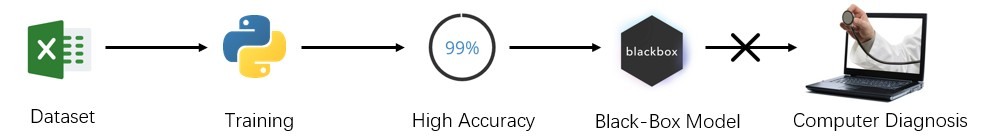
\includegraphics[width=0.8\textwidth]{figures/chapter_defence/interpret.jpg}
% \caption{The workflow of traditional machine learning}
% \label{fig.interpret}
% \end{figure}


% \textbf{Partial Dependence Plot:} Partial Dependence Plots (PDP) reveal the dependence between the target function and target features. The partial function $ \hat{f_{xs}}(x_s) $ is estimated by calculating averages in the training data, also known as the Monte Carlo method. After setting up a grid for features we are interested in (target features), all target features in the training set are modified to be the value at each grid point. Lastly, average prediction at each grid are computed to draw the plot. 

% The drawback of PDP is that one target feature produces 2D plots and two produce 3D plots while it can be pretty hard for a human to understand plots in higher dimensions.

% \begin{equation}
%     \label{eq:1}
% $$\hat{f}_{xs}(x_s) = \frac{1}{n}\sum_{1}^{n}\hat{f}(x_s, x_c^{i})$$
% \end{equation}

% \clearpage

% \textbf{Individual Conditional Expectation: } Individual Conditional Expectation (ICE) is similar to PDP. The difference is that PDP calculates the average over the marginal distribution while ICE keeps them all. Each line in the ICE plot represents predictions for each individual. Without averaging on all instances, ICE unveils heterogeneous relationships but is limited to only one target feature since two features result in overlay surfaces that cannot be identified by human eyes.

% \textbf{Accumulated Local Effects: } Accumulated Local Effects (ALE) averages the changes in the predictions and accumulate them over the local grid. The difference with PDP is that the value at each point of the ALE curve is the difference to the mean prediction calculated in a small window rather than all of the grid. Thus ALE eliminates the effect of correlated features which makes it more suitable in healthcare because it's usually irrational to assume young people having similar physical conditions with the elderly.

% \textbf{Permutation Feature Importance: } The idea behind Permutation Feature Importance is intuitive. A feature is significant for the model if there is a noticeable increase in the model's prediction error after permutation. On the other hand, the feature is less important if the prediction error remains nearly unchanged after shuffling.

% \begin{figure}[H]
% \centering
% 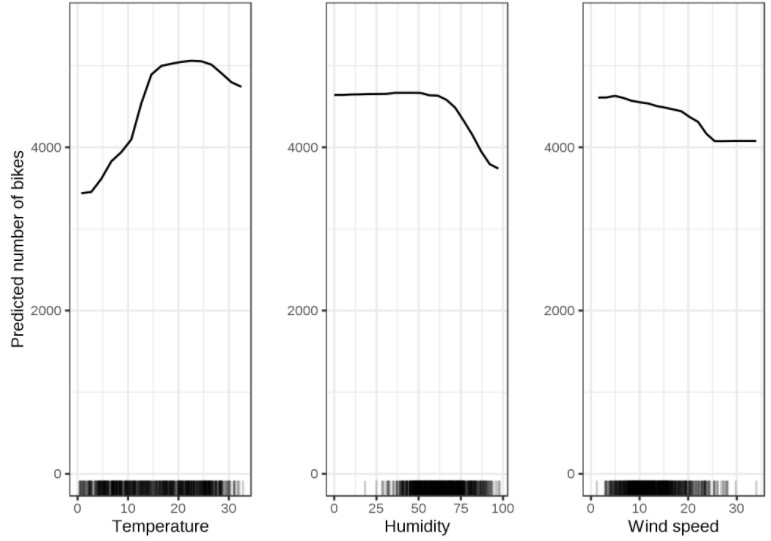
\includegraphics[width=0.7\textwidth]{figures/chapter_defence/pdp.jpg}
% \caption{Partial Dependence Plot that draws the average of predicted value (y axis) if we change target features to be the value at each grid (x axis). For example, if we change all temperatures in the training set to be 20 Celsius, it's predicted that averagely around 5000 bikes will be sold \citep{molnar2019}.}
% \label{fig.pdp}
% \end{figure}

% \begin{figure}[H]
% \centering
% 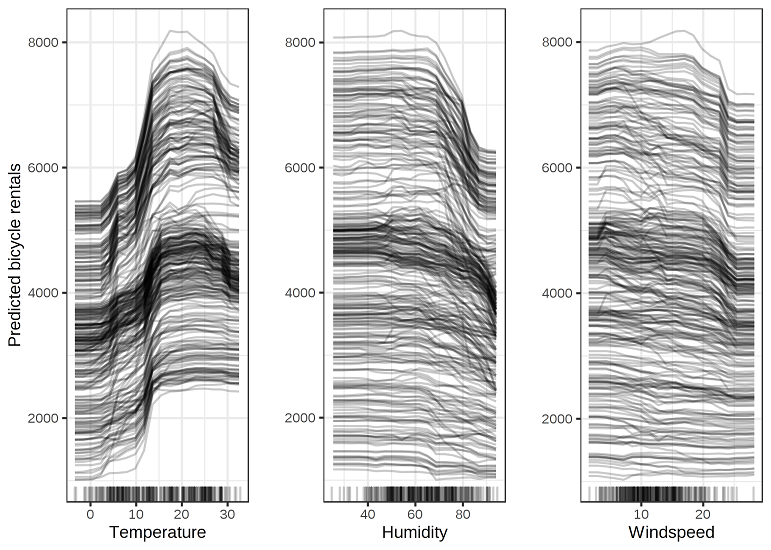
\includegraphics[width=0.7\textwidth]{figures/chapter_defence/ice.png}
% \caption{Individual Conditional Expectation that draws predictions for each individual \citep{molnar2019}.}
% \label{fig.ice}
% \end{figure}

% \begin{figure}[H]
% \centering
% 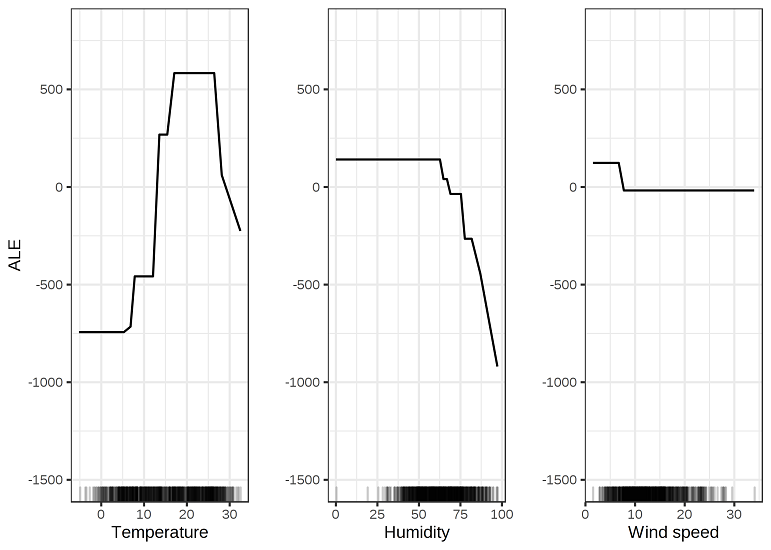
\includegraphics[width=0.7\textwidth]{figures/chapter_defence/ale.png}
% \caption{ALE that draws the difference to the mean prediction calculated \citep{molnar2019}.}
% \label{fig.ale}
% \end{figure}

% \clearpage

% \textbf{Local Interpretable Model-agnostic Explanations:} Local Interpretable Model-agnostic Explanations (LIME) uses interpretable models to approximate the predictions of the original black-box model in specific regions. LIME works for tabular data, text, and images.

% \begin{figure}[H]
% \centering
% 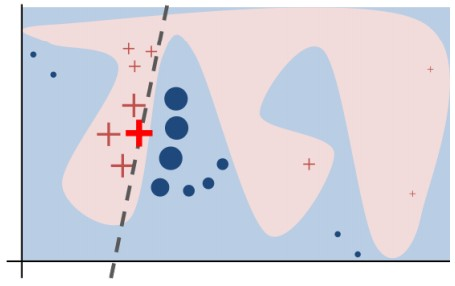
\includegraphics[width=0.4\textwidth]{figures/chapter_defence/lime.jpg}
% \caption{The black-box model’s complex decision function $f$ is approximated by a local model (the dashed line). LIME samples instances, gets predictions using $f$, and weighs them by the proximity to the instance being explained (represented here by size). \citep{ribeiro2016should}}
% \label{fig.lime}
% \end{figure}


% \textbf{Shapley Additive Explanation: } Shapley Additive exPlanation (SHAP) borrows the idea of Shapley value from Game Theory \citep{shapley_1953}, which represents contributions of each player in a game. Calculating Shapley values is computationally expensive when there are hundreds of features, thus Lundberg, Scott M., and Su-In Lee proposed a fast implementation for tree-based models to boost the calculation process \citep{lundberg2017unified}. SHAP has a solid theoretical foundation but is still computationally slow for a lot of instances.

% \begin{figure}[H]
% \centering
% 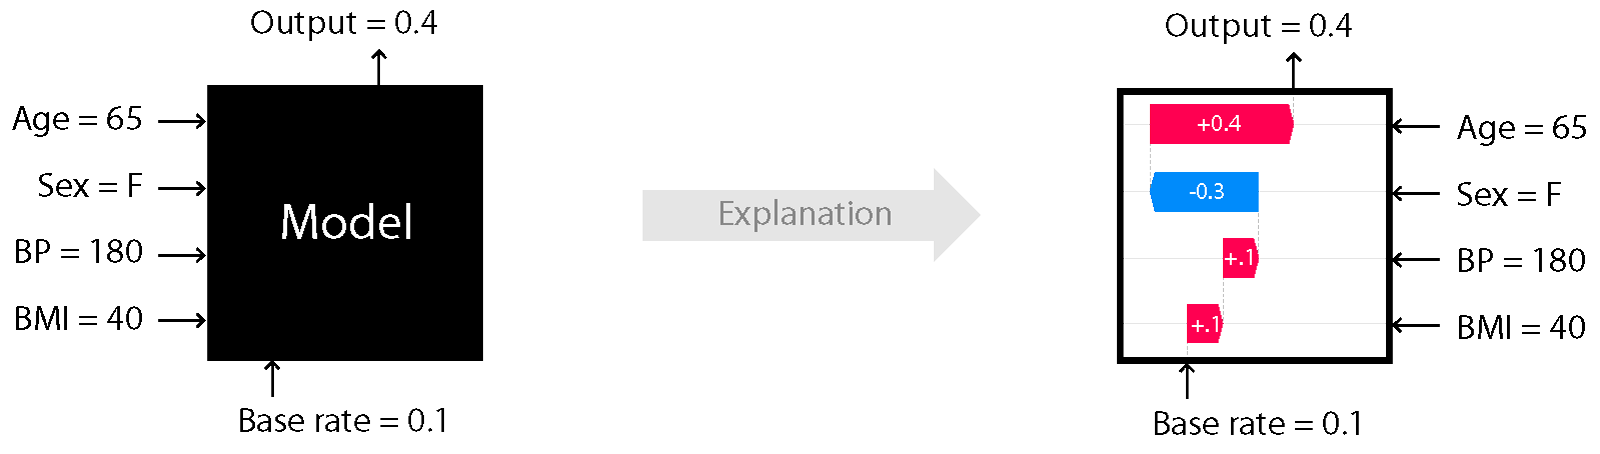
\includegraphics[width=0.9\textwidth]{figures/chapter_defence/shap.png}
% \caption{SHAP \citep{lundberg2017unified}}
% \label{fig.shap}
% \end{figure}

% To summarize, PDP, ICE, and ALE use graphs to visualize the impact of target features while Permutation Feature Importance, LIME, and SHAP provide numerical feature importance that quantitatively ranks the importance of each feature to provide explanations for black-box models.

% Different interpretation methods try to find out the most important features to provide explanations for the output. But as Doshi-Velez and Kim questioned, "Are all models in all defined-to-be-interpretable model classes equally interpretable?"  \citep{doshivelez2017rigorous} And how can we measure the quality of different interpretation methods? 

% % \par
% % To figure out whether those features are correctly ranked, there are two types of indicators for assessment and comparison of explanations: qualitative and quantitative indicators \citep{Carvalho_2019}. Faithfulbess is a qualitative indicator, and monotonicity is a quantitative indicator.

% % \color{blue}
% \textbf{Faithfulness:} Faithfulness incrementally removes each of the attributes deemed important by the interpretability metric, and evaluate the effect on the performance. Then it calculates the correlation between the weights (importance) of the attributes and corresponding model performance and returns correlation between attribute importance weights and the corresponding effect on classifier \citep{alvarezmelis2018robust}.

% \textbf{Monotonicity:} Monotonicity incrementally adds each attribute in order of increasing importance. As each feature is added, the performance of the model should correspondingly increase, thereby resulting in monotonically increasing model performance, and it returns True of False \citep{luss2019generating}.
% \color{black}

% \clearpage

% \section{Defence Techniques}
% \label{sec:defence}

% In previous chapters, we demonstrate that deep neural networks are vulnerable to adversarial attacks. The robustness of deep learning models could even deteriorate after quantization and pruning. Similar to data augmentation, one intuitive solution to this problem is Adversarial Training that incorporates adversarial examples into the training set so that the model can distinguish adversarial examples \citep{goodfellow2015explaining}.

% $$\tilde{J}(\theta, x, y) = \alpha J(\theta, x, y) + (1-\alpha)J(\theta, x+\epsilon sign(\bigtriangledown_{x}J(\theta, x, y)))$$

% On the other hand, we can train a distilled network using Defensive Distillation. In addition to the one-hot encoding of the correct class, if we provide additional information about each class such as probability vectors, the model can extract more information from the training set. A normal DNN is trained using hard class labels (0 or 1) to generate probability vectors that act as soft class labels for the training of the distilled network.

% \begin{figure}[H]
% \centering
% 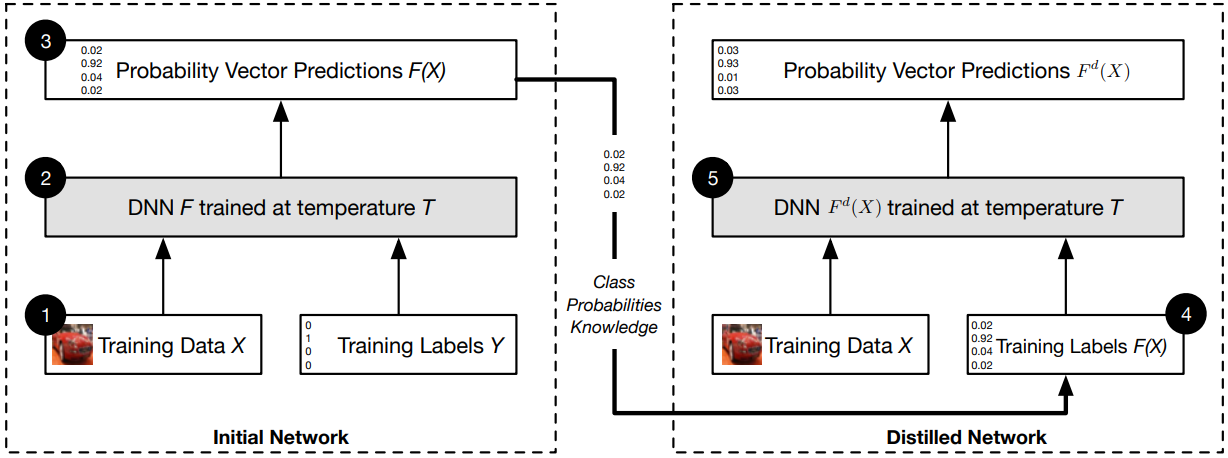
\includegraphics[width=0.6\textwidth]{figures/chapter_defence/defensive_distillation.png}
% \caption{Defensive Distillation \citep{papernot2016distillation}}
% \label{fig.defensive_distillation}
% \end{figure}

% The probability vector $F(X)$ is computed using the following equation:

% $$F(X)=\begin{bmatrix}
% \frac{e^{z_i(X)/T}}{\sum_{l=0}^{N-1}e^{z_l(X)/T}}
% \end{bmatrix}_{i\in 0..N-1}$$

% where $Z(X)=z_0(X), ..., z_{N-1}(X)$ are the N logits corresponding to the hidden layer outputs for each of the N classes in the dataset, and $T$ is a parameter named temperature and shared across the softmax layer. If the temperature is larger than 1, the probability distribution becomes more ambiguous. The temperature is set back to 1 to produce discrete probability predictions.

% In this chapter, we intend to investigate if it's possible to improve the robustness of the model during inference without retraining.

\section{Introduction}

% \begin{figure}[H]
% \setcounter{figure}{3}
% \centering
% 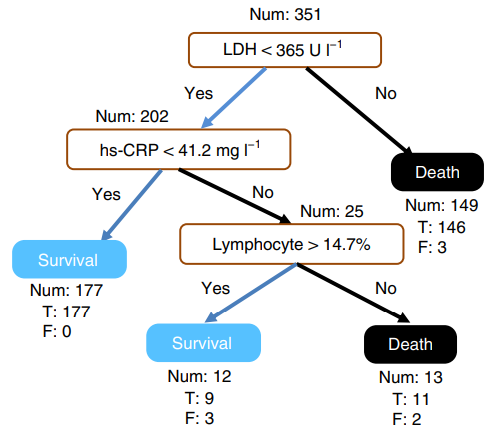
\includegraphics[width=3in]{figures/chapter_interp/nature_dt.png}
% \caption{A decision rule using three key features and their thresholds in
% absolute value. Num, the number of patients in a class; T, the number of
% correctly classified; F, the number of misclassified patients. \citep{Yan2020}}
% \end{figure}

\begin{figure*}
\centering
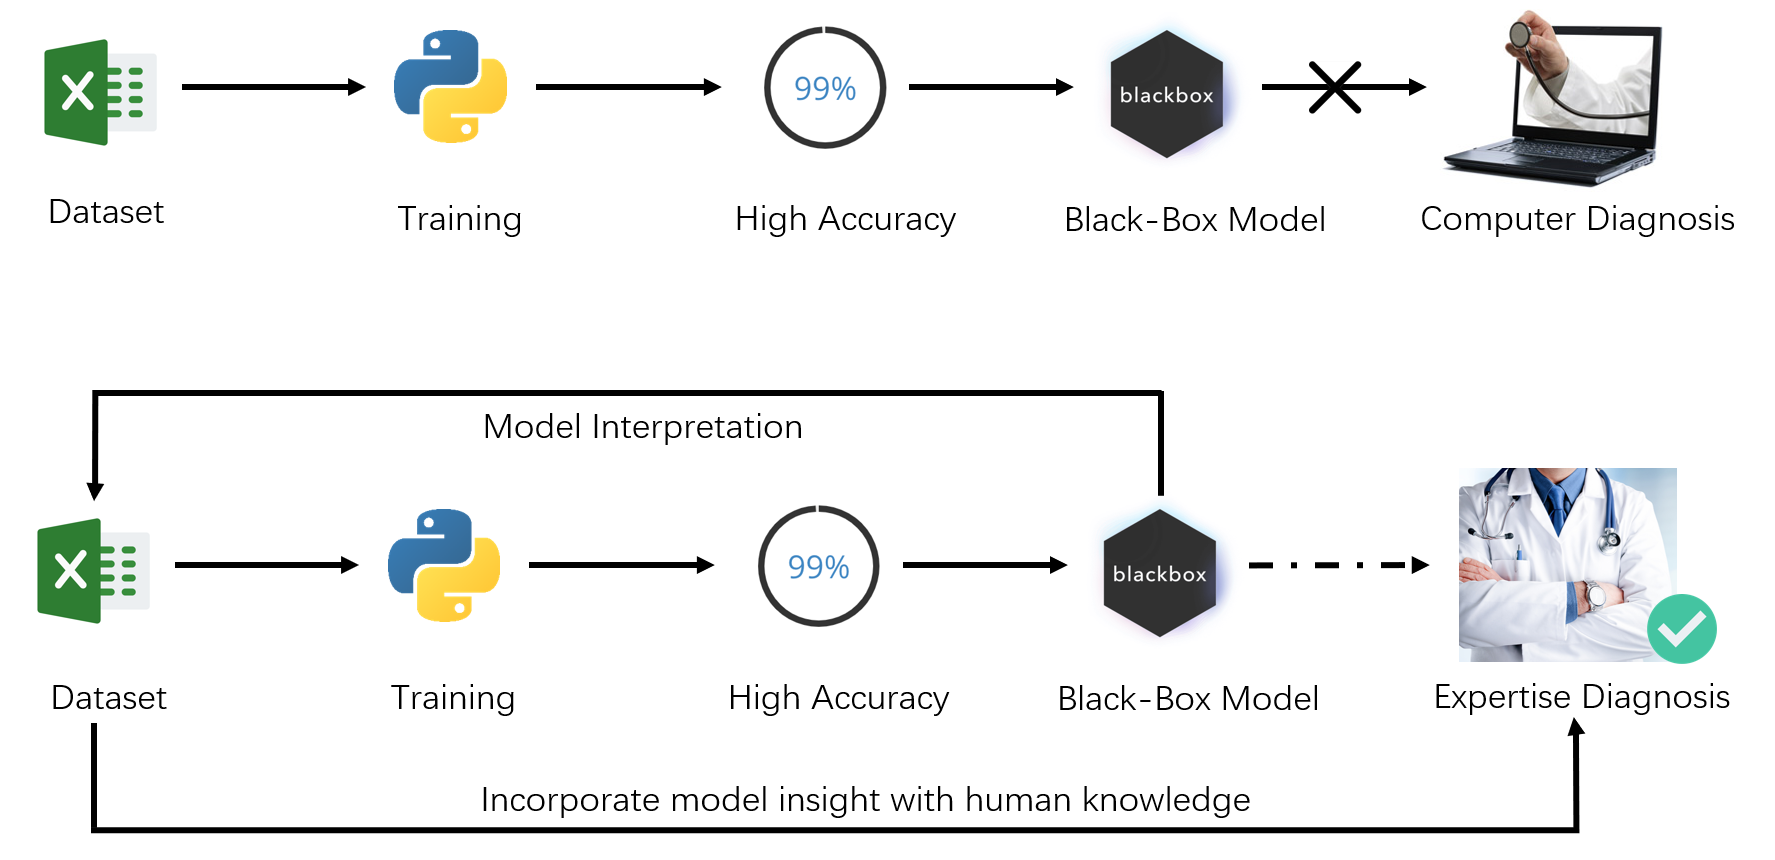
\includegraphics[width=\textwidth]{figures/chapter_interp/interpretable-ml-covid19.png}
\caption{The difference between the usual workflow of machine learning, and our approach.}
\label{fig:approach}
\end{figure*}

% \IEEEPARstart{T}he sudden outbreak of COVID-19 has caused an unprecedented disruption and impact worldwide. With more than 100 million confirmed cases as of February 2021, the pandemic is still accelerating globally. The disease is transmitted by inhalation or contact with infected droplets with an incubation period ranging from 2 to 14 days \citep{singhal2020review}, making it highly infectious and difficult to contain and mitigate.

With the rapid transmission of COVID-19, the demand for medical supplies goes beyond hospitals' capacity in many countries. Various diagnostic and predictive models are employed to release the pressure on healthcare workers. For instance, a deep learning model that detects abnormalities and extract key features of the altered lung parenchyma using chest CT images is proposed \citep{Basu2020Deep}. On the other hand, Rich Caruana et al. exploit intelligible models that use generalized additive models with pairwise interactions to predict the probability of readmission \citep{Caruana2015IntelligibleMF}. To maintain both interpretability and complexity, DeepCOVIDNet is present to achieve predictive surveillance that identifies the most influential features for the prediction of the growth of the pandemic\citep{ramch2020deepcovidnet} through the combination of two modules. The embedding module takes various heterogeneous feature groups as input and outputs an equidimensional embedding corresponding to each feature group. The DeepFM \citep{guo2017deepfm} module computes second and higher-order interactions between them.

% However, deep neural networks are not interpretable due to their complexity which prevents many high-performance models from bring trusted and adopted in healthcare practice. 

% so patterns that do not obey medical knowledge can be recognized and removed. This method is able to scale to large datasets containing hundreds of thousands of patients and thousands of attributes while remaining intelligible and providing accuracy comparable to the best (unintelligible) machine learning methods. But this model is 

Models that achieves high accuracy provide fewer interpretations due to the trade-off between accuracy and interpretability \citep{doshivelez2017rigorous}. To be adopted in healthcare systems that require both interpretability and robustness\citep{goodfellow2014explaining}, the Multi-tree XGBoost algorithm is employed to identify the most significant indicators in COVID-19 diagnosis \citep{Yan2020}. This method exploits the recursive tree-based decision system of the model to achieve high interpretability. On the other hand, a more complex convolutional neural network (CNN) model can discriminates COVID-19 from Non-COVID-19 using chest CT image \citep{matsuyama2020deep}. It achieves interpretability through gradient-weighted class activation mapping to produce a heat map that visually verifies where the CNN model is focusing.

Besides, several model-agnostic methods have been proposed to peek into black-box models, such as \acrfull{pdp} \citep{Friedman2001GreedyFA}, \acrfull{ale} \citep{goldstein2013peeking}, \acrfull{ale} \citep{apley2016visualizing}, \acrfull{pfi} \citep{fisher2018models}, \acrfull{lime} \citep{ribeiro2016i}, \acrfull{shap} \citep{lundberg2017unified}, and Anchors \citep{Ribeiro2018AnchorsHM}. Most of these model-agnostic methods are reasoned qualitatively through illustrative figures and human experiences. To quantitatively measure their interpretability, metrics such as faithfulness \citep{alvarezmelis2018robust} and monotonicity \citep{luss2019generating} are proposed.

In this research, instead of targeting a high-accuracy model, we interpret several models to help medical practitioners promptly discover the most significant biomarkers in the pandemic. Overall, this research makes the following contributions:

\begin{enumerate}
    \item \textbf{Evaluation}: A systematic evaluation of the interpretability of machine learning models that predict the severity level of COVID-19 patients. We experiment with six interpretation methods and two evaluation metrics on our dataset and receive the same result as research that uses a dedicated model. We further validate our approach on a dataset from Kaggle.
    \item \textbf{Implication}: Through the interpretation of models trained on our dataset, we reveal N-Terminal pro-Brain Natriuretic Peptide (NTproBNP), C-Reaction Protein (CRP), lactic dehydrogenase (LDH), and lymphocyte (LYM) as the most indicative biomarkers in identifying patients' severity level. Applying the same approach on the Kaggle dataset, we further unveil three significant features, leukocytes, eosinophils, and platelets.
    \item \textbf{Implementation}: We design a system that healthcare professionals can interact with trained Machine Learning models to incorporate model insights with medical knowledge. We release our implementation, models for future research and validation\footnote{Our source code and models are available on GitHub: \url{https://github.com/wuhanstudio/interpretable-ml-covid-19}.}.
\end{enumerate}

% In this paper, instead of targeting at a high-accuracy model, we use different methods to interpret models which are trained to predict the severity of COVID-19 using a dataset of 92 patient with 74 features. Besides checking whether or not their predictions are based on reasonable medical knowledge, we try to find clues that may be missed by medical practitioners in COVID-19 diagnosis. To quantitatively evaluate different interpretation methods, we use faithfulness and monoticity to justify the interpretation of feature importance. 


% \subsection{Subsection Heading Here}
% Subsection text here.

% needed in second column of first page if using \IEEEpubid
%\IEEEpubidadjcol

% \subsubsection{Subsubsection Heading Here}
% Subsubsection text here.


% An example of a floating figure using the graphicx package.
% Note that \label must occur AFTER (or within) \caption.
% For figures, \caption should occur after the \includegraphics.
% Note that IEEEtran v1.7 and later has special internal code that
% is designed to preserve the operation of \label within \caption
% even when the captionsoff option is in effect. However, because
% of issues like this, it may be the safest practice to put all your
% \label just after \caption rather than within \caption{}.
%
% Reminder: the "draftcls" or "draftclsnofoot", not "draft", class
% option should be used if it is desired that the figures are to be
% displayed while in draft mode.
%
%\begin{figure}[!t]
%\centering
%\includegraphics[width=2.5in]{myfigure}
% where an .eps filename suffix will be assumed under latex, 
% and a .pdf suffix will be assumed for pdflatex; or what has been declared
% via \DeclareGraphicsExtensions.
%\caption{Simulation results for the network.}
%\label{fig_sim}
%\end{figure}

% Note that the IEEE typically puts floats only at the top, even when this
% results in a large percentage of a column being occupied by floats.


% An example of a double column floating figure using two subfigures.
% (The subfig.sty package must be loaded for this to work.)
% The subfigure \label commands are set within each subfloat command,
% and the \label for the overall figure must come after \caption.
% \hfil is used as a separator to get equal spacing.
% Watch out that the combined width of all the subfigures on a 
% line do not exceed the text width or a line break will occur.
%
%\begin{figure*}[!t]
%\centering
%\subfloat[Case I]{\includegraphics[width=2.5in]{box}%
%\label{fig_first_case}}
%\hfil
%\subfloat[Case II]{\includegraphics[width=2.5in]{box}%
%\label{fig_second_case}}
%\caption{Simulation results for the network.}
%\label{fig_sim}
%\end{figure*}
%
% Note that often IEEE papers with subfigures do not employ subfigure
% captions (using the optional argument to \subfloat[]), but instead will
% reference/describe all of them (a), (b), etc., within the main caption.
% Be aware that for subfig.sty to generate the (a), (b), etc., subfigure
% labels, the optional argument to \subfloat must be present. If a
% subcaption is not desired, just leave its contents blank,
% e.g., \subfloat[].


% An example of a floating table. Note that, for IEEE style tables, the
% \caption command should come BEFORE the table and, given that table
% captions serve much like titles, are usually capitalized except for words
% such as a, an, and, as, at, but, by, for, in, nor, of, on, or, the, to
% and up, which are usually not capitalized unless they are the first or
% last word of the caption. Table text will default to \footnotesize as
% the IEEE normally uses this smaller font for tables.
% The \label must come after \caption as always.
%
%\begin{table}[!t]
%% increase table row spacing, adjust to taste
%\renewcommand{\arraystretch}{1.3}
% if using array.sty, it might be a good idea to tweak the value of
% \extrarowheight as needed to properly center the text within the cells
%\caption{An Example of a Table}
%\label{table_example}
%\centering
%% Some packages, such as MDW tools, offer better commands for making tables
%% than the plain LaTeX2e tabular which is used here.
%\begin{tabular}{|c||c|}
%\hline
%One & Two\\
%\hline
%Three & Four\\
%\hline
%\end{tabular}
%\end{table}


% Note that the IEEE does not put floats in the very first column
% - or typically anywhere on the first page for that matter. Also,
% in-text middle ("here") positioning is typically not used, but it
% is allowed and encouraged for Computer Society conferences (but
% not Computer Society journals). Most IEEE journals/conferences use
% top floats exclusively. 
% Note that, LaTeX2e, unlike IEEE journals/conferences, places
% footnotes above bottom floats. This can be corrected via the
% \fnbelowfloat command of the stfloats package.


% \newpage

\section{Preliminary of AI Interpretability}

In this section, six interpretation methods, Partial Dependence Plot, Individual Conditional Expectation, Accumulated Local Effects, Local Interpretable Model-agnostic Explanations, and Shapley Additive Explanation are summarized. We also summarize two evaluation metrics, faithfulness and monotonicity.

\subsection{Model-Agnostic Methods}

In healthcare, restrictions to using only interpretable models bring many limitations in adoption while separating explanations from the model can afford several beneficial flexibilities \citep{ribeiro2016modelagnostic}. As a result, model-agnostic methods have been devised to provide interpretations without knowing model details.

% \par
% Model flexibility: It is often necessary to train models that are accurate for most real-world applications. However, the behavior of high-accuracy models are usually too complex for humans to fully comprehend. Thus, the trade-off between accuracy and interpretability restricts the choice of models in many applications. While model-agnostic methods seperate interpretability from the model thus frees up the model to be as flexible as necessary for the task, enabling the use of any machine learning approach.

% \par
% Explanation flexibility: Interpretable models are limited to certain forms of explanation which is not flexible. For different tasks, it might be useful to have a linear formula in some cases, while a graphic with feature importances can be more favorable under other scenarios. Being model-agnostic, the same model can be explained with different types of explanations, and different degrees of interpretability for each type of explanation \citep{ribeiro2016modelagnostic}.

% \par
% Representation flexibility: Many deep learning models use features that are not perceivable to human to represent input data, such as word embeddings in natural language processing (or NLP) \citep{mikolov2013distributed}. As a result, the explanation system is unable to use a different feature representation as the model being explained. While model-agnostic approaches can generate explanations using different features than the one used by the the original model \citep{ribeiro2016modelagnostic}, thus more flexible.

\textbf{Partial Dependence Plot: } Partial Dependence Plots (PDP) reveal the dependence between the target function and several target features. The partial function $ \hat{f_{xs}}(x_s) $ is estimated by calculating averages in the training data, also known as the Monte Carlo method. After setting up a grid for the features we are interested in (target features), we set all target features in our training set to be the value of grid points, then make predictions and average them all at each grid. The drawback of PDP is that one target feature produces 2D plots and two produce 3D plots while it can be pretty hard for a human to understand plots in higher dimensions.

\begin{equation}
    \label{eq:1}
    \hat{f}_{xs}(x_s) = \frac{1}{n}\sum_{1}^{n}\hat{f}(x_s, x_c^{i})
\end{equation}

\textbf{Individual Conditional Expectation: } Individual Conditional Expectation (ICE) is similar to PDP. The difference is that PDP calculates the average over the marginal distribution while ICE keeps them all. Each line in the ICE plot represents predictions for each individual. Without averaging on all instances, ICE unveils heterogeneous relationships but is limited to only one target feature since two features result in overlay surfaces that cannot be identified by human eyes \citep{molnar2019}.

\textbf{Accumulated Local Effects: } Accumulated Local Effects (ALE) averages the changes in the predictions and accumulate them over the local grid. The difference with PDP is that the value at each point of the ALE curve is the difference to the mean prediction calculated in a small window rather than all of the grid. Thus ALE eliminates the effect of correlated features \citep{molnar2019} which makes it more suitable in healthcare because it's usually irrational to assume young people having similar physical conditions with the elderly.

\begin{equation}    
 \hat{\bar{f}}_{j,ALE}(x) = \sum_{k=1}^{k_j(x)}\frac{1}{n_j(k)}\sum_{i:x_j^{(i)}\in N_j(k)}[f(z_{k,j},x_j^{(i)})-f(z_{k-1,j},x_j^{(i)})] 
\end{equation}
 

\textbf{Permutation Feature Importance: } The idea behind \acrfull{pfi} is intuitive. A feature is significant for the model if there is a noticeable increase in the model's prediction error after permutation. On the other hand, the feature is less important if the prediction error remains nearly unchanged after shuffling.

\textbf{Local Interpretable Model-agnostic Explanations:} Local Interpretable Model-agnostic Explanations (LIME) uses interpretable models to approximate the predictions of the original black-box model in specific regions. LIME works for tabular data, text, and images, but the explanations may not be stable enough for medical applications.

\textbf{Shapley Additive Explanation: } Shapley Additive exPlanation (SHAP) borrows the idea of Shapley value from Game Theory \citep{shapley_1953}, which represents contributions of each player in a game. Calculating Shapley values is computationally expensive when there are hundreds of features, thus Lundberg, Scott M., and Su-In Lee proposed a fast implementation for tree-based models to boost the calculation process \citep{lundberg2017unified}. SHAP has a solid theoretical foundation but is still computationally slow for a lot of instances.

To summarize, PDP, ICE, and ALE only use graphs to visualize the impact of different features while PFI, LIME, and SHAP provide numerical feature importance that quantitatively ranks the importance of each feature.

% \par
% Different methods may understand the same model differently. In healthcare applications, sometimes we can use prior medical knowledge to distinguish reasonable ones, while sometimes it can be cumbersome to sort out most influential ones out of hundreds of features. Thus it is important to find quantitative metrics to evaluate different methods without human intervention.

\subsection{Metrics for Interpretability Evaluation}

Different interpretation methods try to find out the most important features to provide explanations for the output. But as Doshi-Velez and Kim questioned, "Are all models in all defined-to-be-interpretable model classes equally interpretable?"  \citep{doshivelez2017rigorous} And how can we measure the quality of different interpretation methods? 

% \par
% To figure out whether those features are correctly ranked, there are two types of indicators for assessment and comparison of explanations: qualitative and quantitative indicators \citep{Carvalho_2019}. Faithfulbess is a qualitative indicator, and monotonicity is a quantitative indicator.

% \color{blue}
\textbf{Faithfulness:} Faithfulness incrementally removes each of the attributes deemed important by the interpretability metric, and evaluate the effect on the performance. Then it calculates the correlation between the weights (importance) of the attributes and corresponding model performance and returns correlation between attribute importance weights and the corresponding effect on classifier \citep{alvarezmelis2018robust}.

\textbf{Monotonicity:} Monotonicity incrementally adds each attribute in order of increasing importance. As each feature is added, the performance of the model should correspondingly increase, thereby resulting in monotonically increasing model performance, and it returns True of False \citep{luss2019generating}.
\color{black}

In our experiment, both faithfulness and monotonicity are employed to evaluate the interpretation of different machine learning models. 

% \newpage
\section{Empirical Study on COVID}

In this section, features in our raw dataset and procedures of data preprocessing are introduced. After preprocessing, four different models: decision tree, random forest, gradient boosted trees, and neural networks are trained on the dataset. Model interpretation is then employed to understand how different models make predictions, and patients that models make false diagnoses are investigated respectively.

\subsection{Dataset and Pre-processing}

The raw dataset consists of patients with confirmed SARS-CoV-2 laboratory tests between 18th Jan. 2020 and 5th Mar. 2020, in Zhuhai, China. Our Research Ethics Committee waived written informed consent for this retrospective study that evaluated de-identified data and involved no potential risk to patients. All the data of patients have been anonymized before analysis.

% \color{blue}
Tables in the Appendix list all 74 features in the raw dataset consisting of Body Mass Index (BMI), Complete Blood Count (CBC), Blood Biochemical Examination, inflammatory markers, symptoms, anamneses, among others. Whether or not health care professionals will order a test for patients is based on various factors such as medical history, physical examination, and etc. Thus, there is no standard set of tests that are compulsory for every individual which introduces data sparsity. For instance, Left Ventricular Ejection Fraction (LVEF) are mostly empty because most patients are not required to take the color doppler ultrasound test .

\color{black}
After pruning out irrelevant features, such as patients' medical numbers that provide no medical information, and features that have no patients' records (no patient took this test), 86 patients' records with 55 features are selected for further investigation. Among those, 77 records are used for training, cross-validation, and 9 reserved for testing. The feature for classification is Severity01 which indicates normal with 0, and severe with 1. More detailed descriptions about features in our dataset are listed in the Appendix.

Feature engineering is applied before training and interpreting our models, as some features may not provide valuable information or provide redundant information.

First, constant and quasi-constant features were removed. For instance, the two features, PCT2 and Stomachache, have the same value for all patients providing no valuable information in distinguishing normal and severe patients.

% And all the included patients (n=1) with CAD have the comorbidity of arrythmia, so we can remove one of these two features.

Second, correlated features were removed because they provide redundant information. Table \ref{tab:feature_correlation} lists all correlated features using Pearson’s correlation coefficient. 

% We try to understand the strong correlation between two features and remove one of them if necessary.

\begin{table}[H]
\centering
\begin{tabular}{@{}ccc@{}}
\toprule
Feature 1    & Feature 2 & Correlation\\ \midrule
cTnICKMBOrdinal1 & cTnICKMBOrdinal2             & 0.853741       \\
LDH & HBDH             &  0.911419   \\
NEU2           & WBC2             &  0.911419  \\
LYM2       & LYM1             & 0.842688    \\ 
NTproBNP       & N2L2             & 0.808767   \\ 
BMI       & Weight             & 0.842409    \\  
NEU1       & WBC1             & 0.90352    \\  \bottomrule
\end{tabular}
\caption{Feature Correlation}
\label{tab:feature_correlation}
\end{table}


\begin{enumerate}  
\item There is strong correlation between cTnICKMBOrdinal1 and cTnICKMBOrdinal2 because they are the same test among a short range of time which is the same for LYM1 and LYM2.
\item LDH and HBDH levels are significantly correlated with heart diseases, and the HBDH/LDH ratio can be calculated to differentiate between liver and heart diseases.
\item Neutrophils (NEU1/NEU2) are all correlated to the immune system. In fact, most of the white blood cells that lead the immune system’s response are neutrophils. Thus, there is a strong correlation between NEU1 and WBC1, NEU2 and WBC2.
\item In the original dataset, there is no much information about N2L2 which is correlated with NTproBNP, thus NTproBNP remains.
\item the correlation between BMI and weight is straight forward because Body Mass Index (BMI) is a person’s weight in kilograms divided by the square of height in meters.
\end{enumerate}

Third, statistical methods that calculate mutual information is employed to remove features with redundant information.

\begin{table}[H]
\centering
\begin{tabular}{@{}cc@{}}
\toprule
Statistical Methods & Removed Features \\ \midrule
Mutual Information & Height, CK, HiCKMB, Cr, WBC1, Hemoptysis      \\
Univariate & Weight, AST, CKMB, PCT1, WBC2        \\  \bottomrule
\end{tabular}
\caption{Features with Mutual Information}
\end{table}

Mutual information is calculated using equation \ref{eq:2} that determines how similar the joint distribution p(X, Y) is to the products of individual distributions p(X)p(Y). Univariate Test measures the dependence of two variables, and a high p-value indicates a less similar distribution between X and Y. 

\begin{equation}
    I(X;Y)=\sum_{x,y}p(x, y)log\frac{p(x,y)}{p(x)p(y)} \label{eq:2}
\end{equation}

\par
After feature engineering, there are 37 features left for training and testing.

\subsection{Training Models}

Machine learning models outperform humans in many different areas in terms of accuracy. Interpretable models such as the decision tree are easy to understand, but not suitable for large scale applications. Complex models achieve high accuracy while giving less explanation. 

For healthcare applications, both accuracy and interpretability are significant. Four different models are selected to extract information from our dataset: Decision Tree, Random Forests, Gradient Boosted Trees, and Neural Networks.

\begin{table}[H]
\centering
\begin{tabular}{@{}ccc@{}}
\toprule
Layer Type   & Output Shape & Param \\ \midrule
Dense & (None, 10) & 370           \\
Dropout & (None, 10) & 0           \\
Dense & (None, 15) & 165           \\
Dropout & (None, 15) & 0           \\
Dense & (None, 5) & 80           \\
Dropout & (None, 5) & 0           \\
Dense & (None, 1) & 6           \\
\bottomrule
\end{tabular}
\caption{The structure of Neural Networks}
\label{tab:nn}
\end{table}

\textbf{Decision Tree:} Decision Tree (DT) is a widely adopted method for both classification and regression. It's a non-parametric supervised learning method that infers decision rules from data features. The decision tree try to find decision rules that make the best split measured by Gini impurity or entropy. More importantly, the generated decision tree can be visualized, thus easy to understand and interpret \citep{Breiman2015Classification}.

\textbf{Random Forest:} Random Forests (RF) is a kind of ensemble learning method \citep{Breiman2001Random} that employs bagging strategy. Multiple decision trees are trained using the same learning algorithm, and then predictions are aggregated from the individual decision tree. Random forests produce great results most of the time even without much hyper-parameter tuning. As a result, it has been widely accepted for its simplicity and good performance. However, it is rather difficult for humans to interpret hundreds of decision trees, so the model itself is less interpretable than a single decision tree.

\textbf{Gradient Boosted Trees:} Gradient Boosted Trees is another ensemble learning method that employs boosting strategy \citep{gbtrees}. Through sequentially adding one decision tree at one time, gradient boosted trees combine results along the way. With fine-tuned parameters, gradient boosting can result in better performance than random forests. Still, it is tough for humans to interpret a sequence of decision trees and thus considered as black-box models.

\textbf{Neural Networks:} Neural Networks could be the most promising model in achieving a high accuracy and even outperforms humans in medical imaging \citep{maier2018gentle}. Though the whole network is difficult to understand, deep neural networks are stacks of simple layers, thus can be partially understood through visualizing outputs of intermediate layers \citep{Montavon_2018}.

% \par 
%  Simple interpretable models cannot achieve satisfactory accuracy in applications of image, thus many model-agnostic methods are employed to interpret complex black-box models.

As for the implementation, there is no hyperparameter for the decision tree. For random forests, 100 trees are used during the initialization. The hyperparameters for gradient boosted trees are selected according to prior experience. The structure for neural networks is listed in table \ref{tab:nn}. All these methods are implemented using scikit-learn \citep{scikit-learn}, Keras and Python3.6.

After training, gradient boosted trees and neural networks achieve the highest precision on the test set. Among 9 patients in our test set, four of them are severe. Both the decision tree and random forests fail to identify two severe patients, while Gradient Boosted Trees and Neural Networks find all of the severe patients. 


\begin{table}[H]
\centering
\begin{tabular}{cccccc}
\toprule
Classifier    & CV & \multicolumn{3}{c}{Test Set} & 95\% CI \\ \midrule
                        & F1     & Precision  & Recall  & F1    &\\
Decision Tree           & 0.55   & 0.67       & 0.50    & 0.57  & 0.31\\
Random Forest           & 0.62   & 0.67       & 0.50    & 0.57  & 0.31\\
Gradient Boosted Trees  & 0.67   & 0.78       & 1.00    & 0.80  & 0.27\\
Neural Networks         & 0.58   & 0.78       & 1.00    & 0.80  & 0.27\\ \bottomrule
\end{tabular}
\caption{Classification Results on our dataset}
\end{table}

% \par
% In this paper, we do not try to get the most accurate model, instead we focus on understanding different models. Thus, in the next section, we'll interpret these models and try to understand why they make different decisions.

% \newpage
\subsection{Interpretation (Permutation Feature Importance)}

First, we use  Permutation Feature Importance to find the most important features in different models. In table \ref{tab:important_feature}, CRP2 and NTproBNP are recognized as most important features by most models.

\begin{table}[H]
\centering
\begin{tabular}{@{}ccc@{}}
\toprule
Model                   & Most Important Features \\ \midrule
Decision Tree           & NTproBNP, CRP2, ALB2, Temp, Symptom      \\
Random Forest           & CRP2, NTproBNP, cTnI, LYM1, ALB2         \\
Gradient Boosted Trees  & CRP2, cTnITimes, LYM1, NTproBNP, Phlegm  \\
Neural Networks         & NTproBNP, CRP2, CRP1, LDH, Age           \\  \bottomrule
\end{tabular}
\caption{Five most important features}
\label{tab:important_feature}
\end{table}

According to medical knowledge, CRP refers to C-Reactive Protein, which increases when there's inflammation or viral infection in the body. C-reactive protein (CRP) levels are positively correlated with lung lesions and could reflect disease severity\citep{WANG2020332}. NTproBNP refers to N-Terminal prohormone of Brain Natriuretic Peptide, which will be released in response to changes in pressure inside the heart. The CRP level in severe patients rises due to viral infection, and patients with higher NT-proBNP (above 88.64 pg/mL) level had more risks of in-hospital death \citep{Gao2020.03.07.20031575}.

% Thus, the two most important features revealed by machine learning models do not obey medical knowledge.

% \clearpage

\subsection{Interpretation (PDP, ICE, ALE)}

After recognizing the most important features, PDP, ICE, and ALE are employed to further visualize the relationship between CRP and NTproBNP.

In the PDPs, all of the four models indicate a higher risk of turning severe with the increase of NTproBNP and CRP which is consistent with the retrospective study on COVID-19. The difference is that different models have different tolerances and dependence on NTproBNP and CRP. Averagely, the decision tree has less tolerance on a high level of NTproBNP ($>$2000ng/ml), and gradient boosted trees give a much higher probability of death as CRP increases. Since PDPs only calculate an average of all instances, we use ICEs to identify heterogeneity.

\begin{figure}[H]
\centering
\begin{subfigure}[b]{0.85\textwidth}
    \centering
    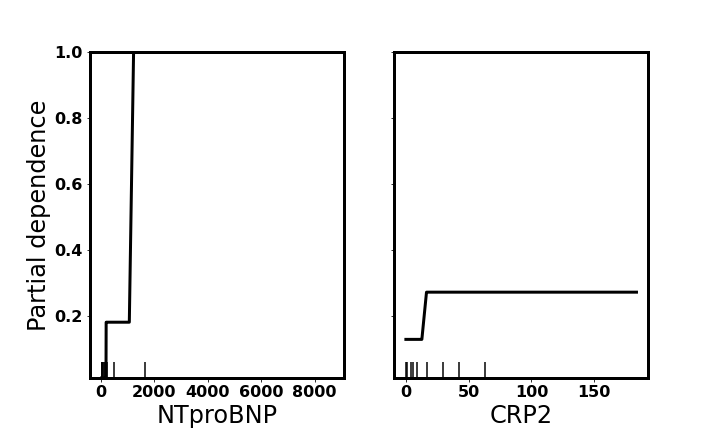
\includegraphics[width=\textwidth]{figures/chapter_interp/dt_pdp_crp_ntproBNP.png}
    \caption{Decision Tree}
    \label{fig:dt_pdp}
\end{subfigure}
% \hfill
\begin{subfigure}[b]{0.85\textwidth}
    \centering
    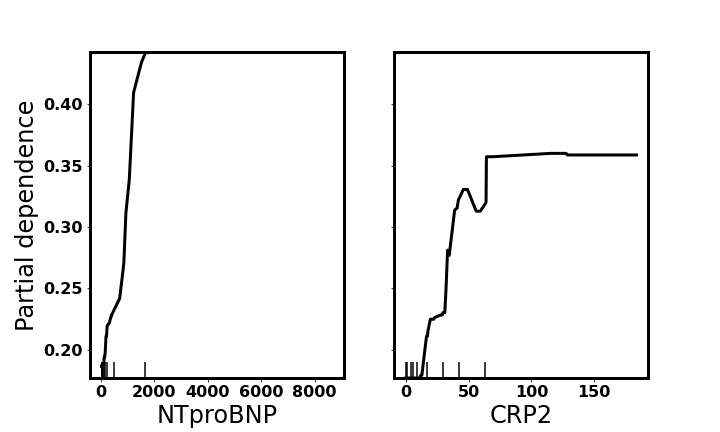
\includegraphics[width=\textwidth]{figures/chapter_interp/rf_pdp_crp_ntproBNP.png}
    \caption{Random Forest}
    \label{fig:rf_pdp}
\end{subfigure}
% \vskip\baselineskip
% \hfill
\end{figure}
\begin{figure}[H]\ContinuedFloat
\centering
\begin{subfigure}[b]{0.85\textwidth}
    \centering
    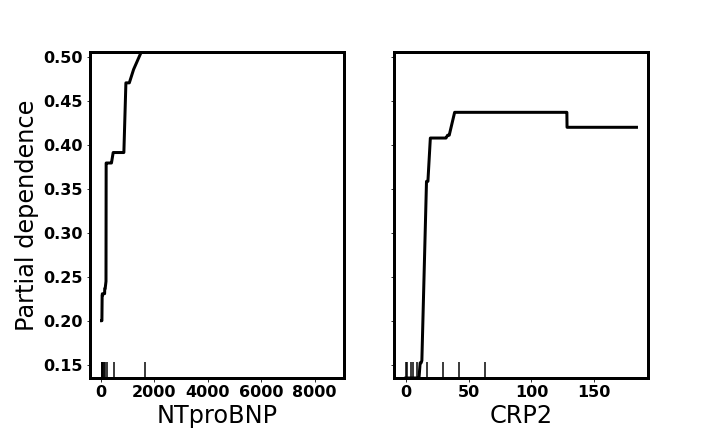
\includegraphics[width=\textwidth]{figures/chapter_interp/xgbc_pdp_crp_ntproBNP.png}
    \caption{Gradient Boosted Trees}
    \label{fig:gbt_pdp}
\end{subfigure}
% \hfill
\begin{subfigure}[b]{0.85\textwidth}
    \centering
    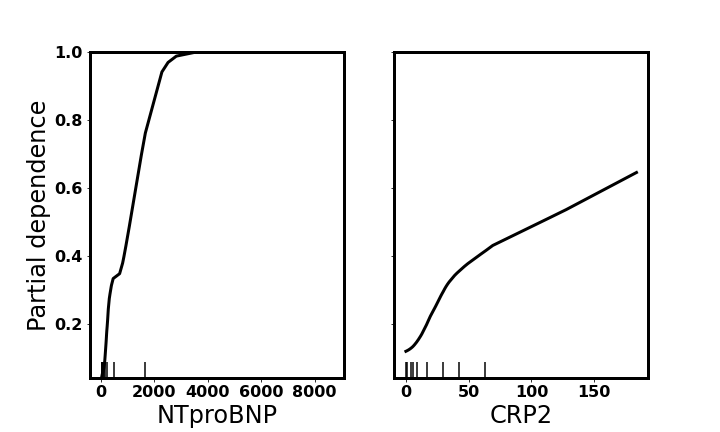
\includegraphics[width=\textwidth]{figures/chapter_interp/nn_pdp_crp_ntproBNP.png}
    \caption{Neural Networks}
    \label{fig:nn_pdp}
\end{subfigure}
\caption{Partial Dependence Plot: There is a positive correlation between the level of NTproBNP/CRP and the probability of turning severe because as NTproBNP/CRP increases, the average possibility (y-axis) of turning severe increases.}
\label{fig.pdp}
\end{figure}

ICE reveals individual differences. Though all of the models give a prediction of a higher risk of severe as NTproBNP and CRP increase, some patients have a much higher initial probability which indicates other features have an impact on overall predictions. For example, elderly people have higher NTproBNP than young people and have a higher risk of turning severe.

In the ALEs,  as NTproBNP and CRP get higher, all of the four models give a more positive prediction of turning severe, which coincides with medical knowledge.

\clearpage

\null
\vfill

\begin{figure}[H]
\centering
\begin{subfigure}[b]{\textwidth}
    \centering
    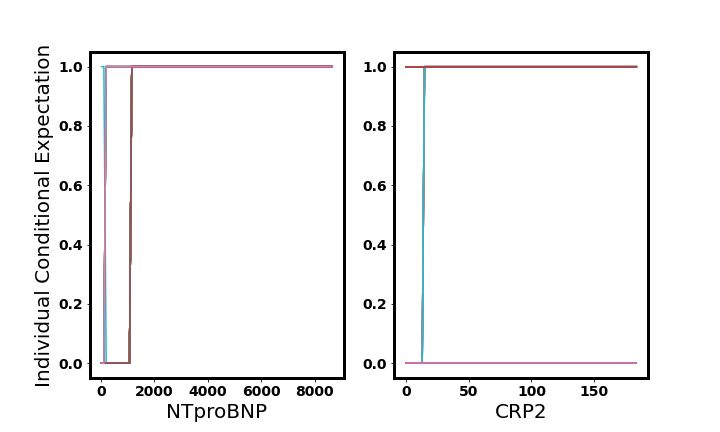
\includegraphics[width=\textwidth]{figures/chapter_interp/dt_ice_crp_ntproBNP.png}
    \caption{Decision Tree}
    \label{fig:dt_ice}
\end{subfigure}
\hfill
\begin{subfigure}[b]{\textwidth}
    \centering
    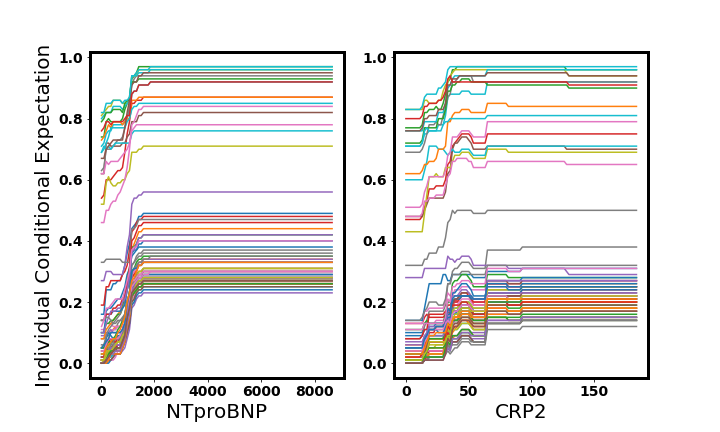
\includegraphics[width=\textwidth]{figures/chapter_interp/rf_ice_crp_ntproBNP.png}
    \caption{Random Forest}
    \label{fig:rf_ice}
\end{subfigure}
\hfill
\end{figure}

\vfill

\clearpage

\null
\vfill

\begin{figure}[H] \ContinuedFloat
% \vskip\baselineskip
\begin{subfigure}[b]{\textwidth}
    \centering
    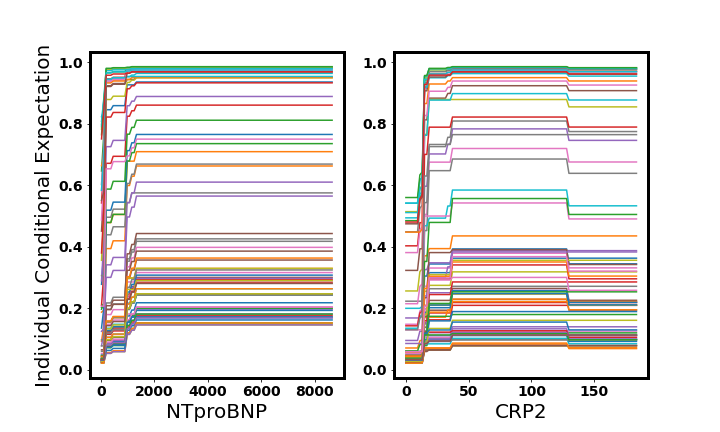
\includegraphics[width=\textwidth]{figures/chapter_interp/xgbc_ice_crp_ntproBNP.png}
    \caption{Gradient Boosted Trees}
    \label{fig:gbt_ice}
\end{subfigure}
\hfill
\begin{subfigure}[b]{\textwidth}
    \centering
    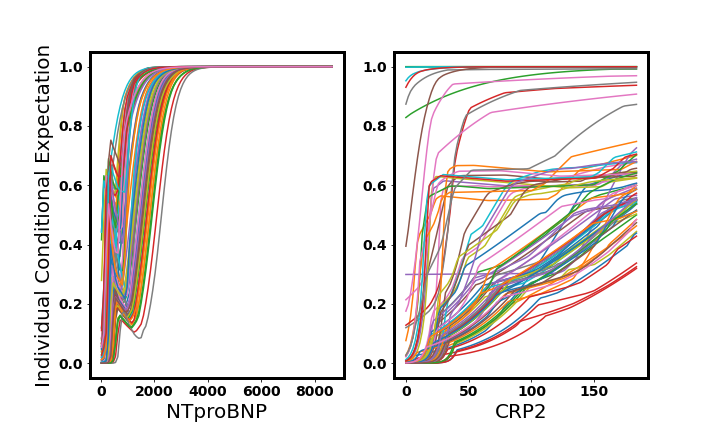
\includegraphics[width=\textwidth]{figures/chapter_interp/nn_ice_crp_ntproBNP.png}
    \caption{Neural Networks}
    \label{fig:nn_ice}
\end{subfigure}
\caption{Individual Conditional Expectation: Each line in different colors represents a patient. As we increase NTproBNP/CRP while keeping other features the same, the probability of turning severe increases for each individual, but each patient has a different starting level because their other physical conditions differ.}
\label{fig.ice}
\end{figure}

\vfill

% \par
% Sometimes it's not appropriate to use PDP and ICE in medical applications, because both PDP and ICE sample in a grid and make predictions, while some points in the grid may never appear in real world. For example, it's very rare for young people to have a NTproBNP as high as elderlys. ALE only samples in a small range of area which makes it more realistic.

\clearpage

\null
\vfill

\begin{figure}[H]
\centering
\begin{subfigure}[b]{\textwidth}
    \centering
    \includegraphics[width=\textwidth]{figures/chapter_interp/dt_ALE_NTproBNP_CRP.png}
    \caption{Decision Tree}
    \label{fig:dt_ale}
\end{subfigure}
\hfill
\begin{subfigure}[b]{\textwidth}
    \centering
    \includegraphics[width=\textwidth]{figures/chapter_interp/rf_ALE_NTproBNP_CRP.png}
    \caption{Random Forest}
    \label{fig:rf_ale}
\end{subfigure}
\hfill
% \vskip\baselineskip
\end{figure}

\vfill

\clearpage

\null
\vfill

\begin{figure}[H] \ContinuedFloat
\begin{subfigure}[b]{\textwidth}
    \centering
    \includegraphics[width=\textwidth]{figures/chapter_interp/xgbc_ALE_NTproBNP_CRP.png}
    \caption{Gradient Boosted Trees}
    \label{fig:gbt_ale}
\end{subfigure}
\hfill
\begin{subfigure}[b]{\textwidth}
    \centering
    \includegraphics[width=\textwidth]{figures/chapter_interp/nn_ALE_NTproBNP_CRP.png}
    \caption{Neural Networks}
    \label{fig:nn_ale}
\end{subfigure}
\caption{Accumulated Local Effects: As the level of NTproBNP/CRP increases, the possibility of turning severe (yellow) goes above the average.}
\label{fig.ale}
\end{figure}

\vfill

\clearpage

\subsection{Misclassified Patients}

Even though the most important features revealed by our models exhibit medical meaning, some severe patients fail to be recognized. Both Gradient Boosted Trees and Neural Networks recognize all severe patients and yield a recall of 1.00, while the decision tree and random forests fail to reveal two of them. 

Patient No. 2 (normal) is predicted with a probability of 0.53 of turning severe which is around the boundary (0.5). While for patient No. 5 (severe), the model gives a relatively low probability of turning severe (0.24).

\begin{table}[H]
\centering
\begin{tabular}{ccccc}
\toprule
No & Class  & Probability of Severe & Prediction & Type\\ \midrule
2 & Normal & 0.53 & Severe & \textbf{False Positive}       \\
5 & Severe & 0.24  & Normal & \textbf{False Negative}   \\ \bottomrule
\end{tabular}
\caption{Misclassified Patients}
\label{tab:misclassified}
\end{table}

% \clearpage
\subsection{Interpretation (False Negative)}

Suppose different models represent different doctors, then the decision tree and random forests make the wrong diagnosis for patient no. 5. The reason human doctors classified the patient as severe is that he actually needed a respirator to survive. To further investigate why the decision tree and random forests make wrong predictions, Local Interpretable Model-agnostic Explanations (LIME) and (Shapley Additive Explanation) SHAP are employed.

LIME: Features in green have a positive contribution to the prediction (increasing the probability of turning severe), and features in red have a negative effect on the prediction (decreasing the probability of turning severe).

SHAP: Features pushing the prediction to be higher (severe) are shown in red,  and those pushing the prediction to be lower (normal) are in blue.


\subsubsection{\textbf{Wrong Diagnoses}}

Take the decision tree as an example, in the figure \ref{fig:lime_dt_5}, the explanation by LIME illustrates that NTproBNP and CRP are two features (in green) that have a positive impact on the probability of turning severe. Even though patient No.5 is indeed severe, the decision tree gives an overall prediction of normal (false negative). Thus, we would like to investigate features that have a negative impact on the probability of turning severe.

In the figure \ref{fig:shap_xgbc_5}, the explanation by SHAP reveals that the patient is diagnosed as normal by the decision tree because the patient has no symptom. Even though the patient has a high NTproBNP and CRP, having no symptom makes it less likely to classify him as severe. The record was taken when the patient came to the hospital for the first time. It is likely that the patient developed symptoms later and turned severe.

However, both gradient boosted trees and neural networks are not deceived by the fact the patient has no symptom. Their predictions indicate that the patient is likely to turn severe in the future.

\subsubsection{Correct Diagnoses}

In the figure \ref{fig:shap_xgbc_5} and figure \ref{fig:shap_nn_5}, gradient boosted trees and neural networks do not prioritise the feature symptom. They put more weight on test results (NTproBNP and CRP). Thus they make correct predictions based on the fact that the patient's test results are serious.

Besides, neural networks notice that the patient is elderly (Age = 63). If we calculate the average age in different severity levels, it is noticeable that elderly people are more likely to deteriorate.

\begin{table}[H]
\centering
\begin{tabular}{@{}cc@{}}
\toprule
Severity Level   & Average Age\\ 
\midrule
0      &          36.83 \\ 
1      &          47.45 \\ 
2      &          54.31 \\ 
3      &          69.40 \\ 
\bottomrule
\end{tabular}
\caption{Average Age in different severity levels}
\end{table}


Gradient boosted trees and neural networks make correct predictions because they trust more in test results, while the decision tree relies more on whether or not a patient has symptoms. As a result, gradient boosted trees and neural networks are capable of recognizing patients that are likely to turn severe in the future while the decision tree makes predictions relying more on patients' current situation.

% \color{blue}
Medical research is a case-by-case study. Every patient is unique. It's strenuous to find a single criterion that suits every patient, thus it's important to focus on each patient and make a diagnosis accordingly. This is one of the benefits of using interpretable machine learning. It unveils the most significant features for most patients and provides the interpretation for each patient as well.
% \color{black}

\clearpage

\null
\vfill

\begin{figure}[H]
% \setcounter{figure}{4}
\centering
\begin{subfigure}[b]{\textwidth}
    \centering
    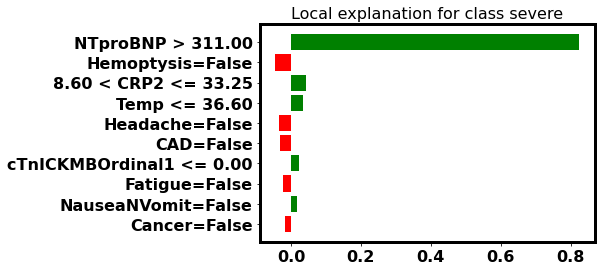
\includegraphics[width=\textwidth]{figures/chapter_interp/lime_dt_5.png}
    \caption{Decision Tree}
    \label{fig:lime_dt_5}
\end{subfigure}
\hfill
\begin{subfigure}[b]{\textwidth}
    \centering
    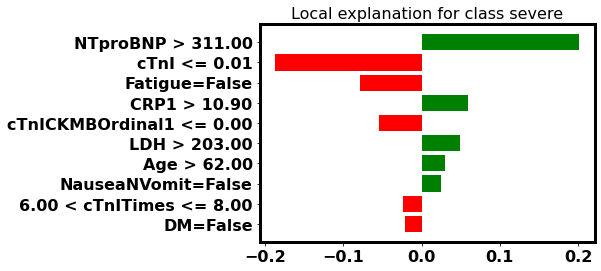
\includegraphics[width=\textwidth]{figures/chapter_interp/lime_rf_5.png}
    \caption{Random Forests}
    \label{fig:lime_rf_5}
\end{subfigure}
\hfill
\end{figure}

\vfill

\clearpage

\null
\vfill

\begin{figure}[H] \ContinuedFloat
\begin{subfigure}[b]{\textwidth}
    \centering
    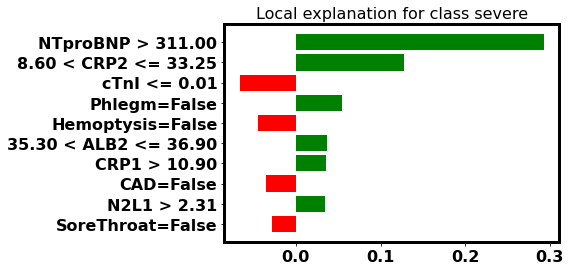
\includegraphics[width=\textwidth]{figures/chapter_interp/lime_xgbc_5.png}
    \caption{Gradient Boosted Trees}
    \label{fig:lime_xgbc_5}
\end{subfigure}
\hfill
\begin{subfigure}[b]{\textwidth}
    \centering
    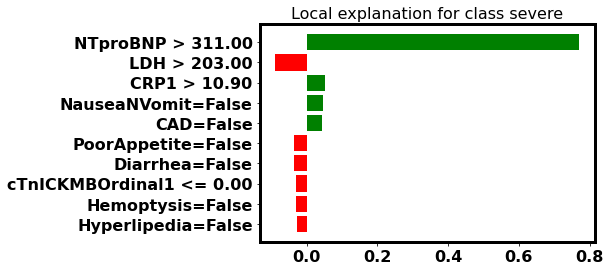
\includegraphics[width=\textwidth]{figures/chapter_interp/lime_nn_5.png}
    \caption{Neural Networks}
    \label{fig:lime_nn_5}
\end{subfigure}
\caption{LIME Explanation (\textbf{False-Negative Patient No.5}): Features in green have a positive contribution to the prediction (increasing the probability of turning severe), and features in red have a negative effect on the prediction (decreasing the probability of turning severe)}
\label{fig:lime_5}
\end{figure}

\vfill

\clearpage

% \null
% \vfill

% \begin{figure}[H]
% % \setcounter{figure}{5}
% \centering
% \begin{subfigure}[b]{}
%     \centering
%     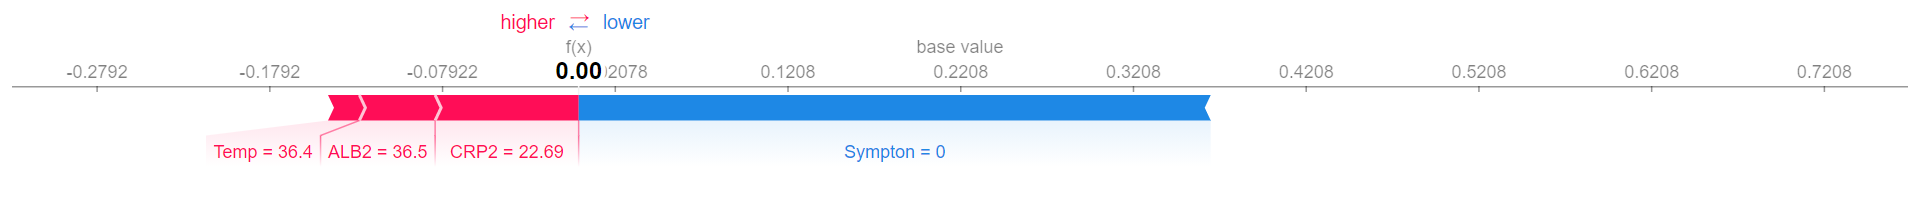
\includegraphics[angle=90,origin=c]{figures/chapter_interp/shap_dt_5.png}
%     \caption{Decision Tree}
%     \label{fig:shap_dt_5}
% \end{subfigure}
% \hfill
% \begin{subfigure}[b]{}
%     \centering
%     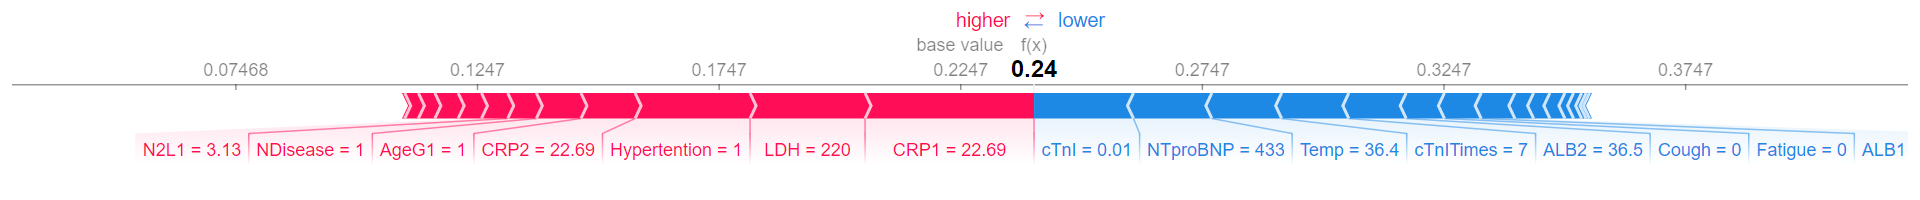
\includegraphics[angle=90,origin=c]{figures/chapter_interp/shap_rf_5.png}
%     \caption{Random Forests}
%     \label{fig:shap_rf_5}
% \end{subfigure}
% \vfill
% \begin{subfigure}[b]{}
%     \centering
%     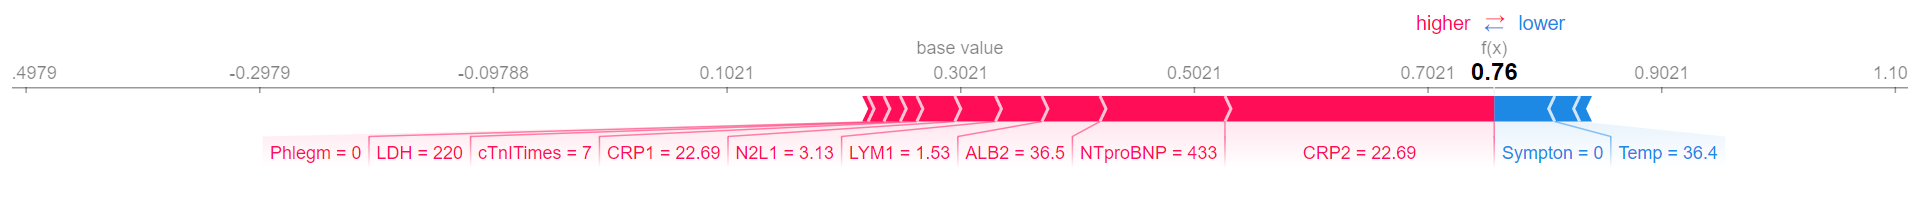
\includegraphics[angle=90,origin=c]{figures/chapter_interp/shap_xgbc_5.png}
%     \caption{Gradient Boosted Trees}
%     \label{fig:shap_xgbc_5}
% \end{subfigure}
% \vfill
% \begin{subfigure}[b]{}
%     \centering
%     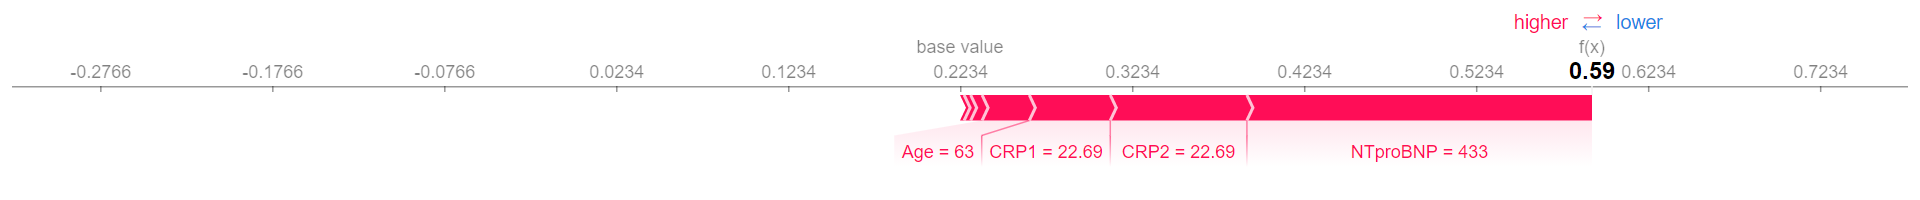
\includegraphics[angle=90,origin=c]{figures/chapter_interp/shap_nn_5.png}
%     \caption{Neural Networks}
%     \label{fig:shap_nn_5}
% \end{subfigure}
% \vfill
% \caption{SHAP Explanation (\textbf{False-Negative Patient No.5}): Features pushing the prediction to be higher (severe) are shown in red,  and those pushing the prediction to be lower (normal) are in blue.}
% \label{fig:shap_5}
% \end{figure}

\begin{sidewaysfigure}
    \centering
    \begin{subfigure}[b]{\textheight}
        \centering
        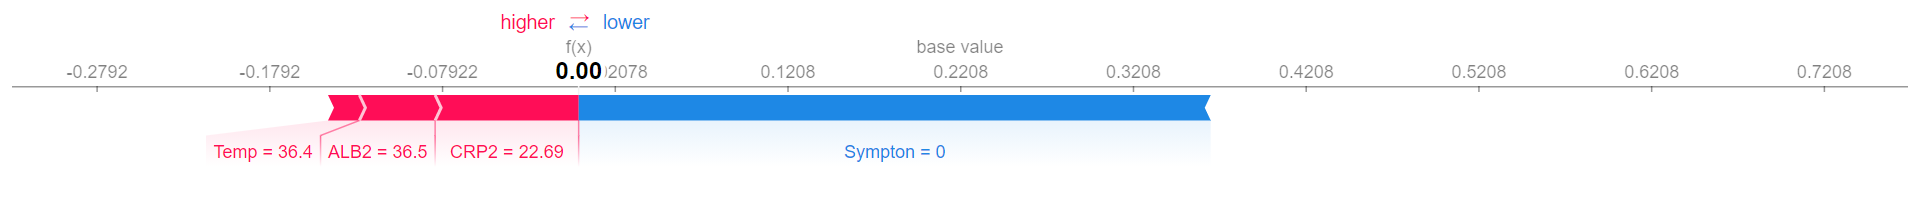
\includegraphics[width=\textheight]{figures/chapter_interp/shap_dt_5.png}
        \caption{Decision Tree}
        \label{fig:shap_dt_5}
    \end{subfigure}
    \vfill
    \begin{subfigure}[b]{\textheight}
        \centering
        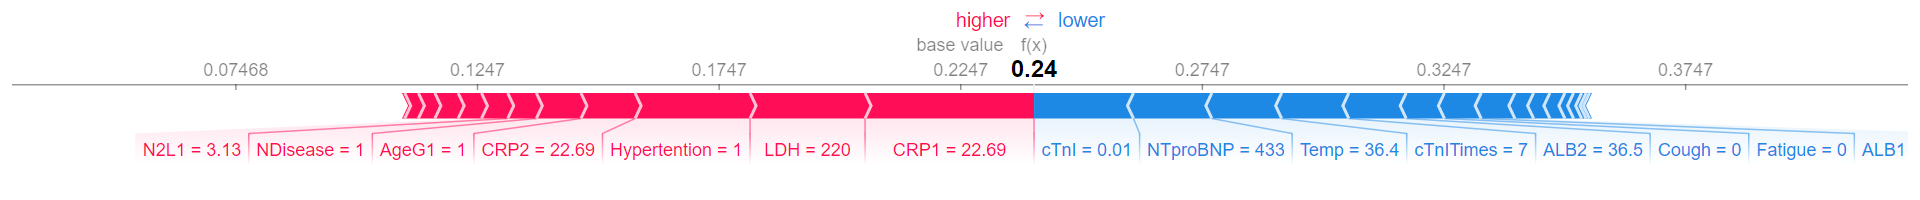
\includegraphics[width=\textheight]{figures/chapter_interp/shap_rf_5.png}
        \caption{Random Forests}
        \label{fig:shap_rf_5}
    \end{subfigure}
    \vfill
    \begin{subfigure}[b]{\textheight}
        \centering
        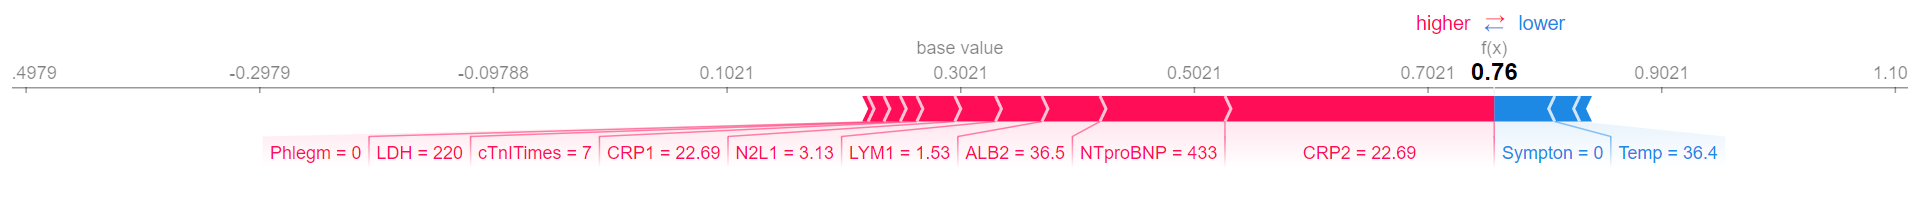
\includegraphics[width=\textheight]{figures/chapter_interp/shap_xgbc_5.png}
        \caption{Gradient Boosted Trees}
        \label{fig:shap_xgbc_5}
    \end{subfigure}
    \vfill
    \begin{subfigure}[b]{\textheight}
        \centering
        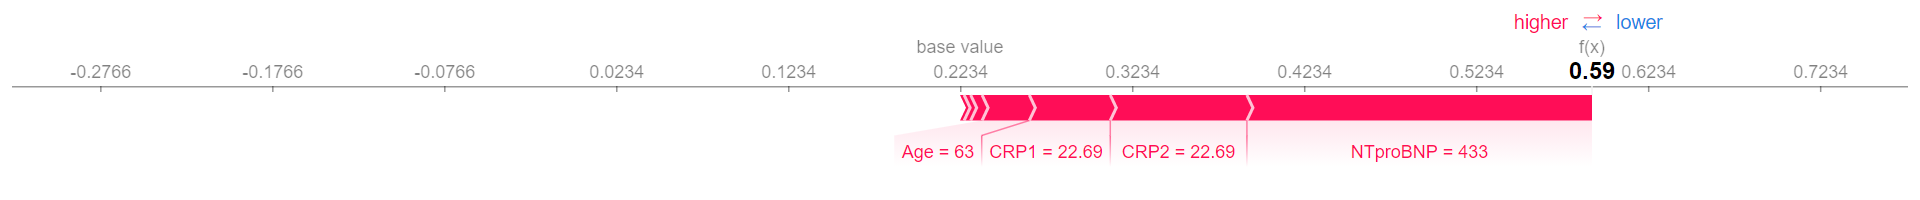
\includegraphics[width=\textheight]{figures/chapter_interp/shap_nn_5.png}
        \caption{Neural Networks}
        \label{fig:shap_nn_5}
    \end{subfigure}
  \caption{SHAP Explanation (\textbf{False-Negative Patient No.5}): Features pushing the prediction to be higher (severe) are shown in red, and those pushing the prediction to be lower (normal) are in blue.}
  \label{fig:shap_5}
\end{sidewaysfigure}


% \vfill

\clearpage

\subsection{Interpretation (False Positive)}

With limited medical resources at the initial outbreak of the pandemic, it's equally important to investigate false positive, so that valuable resources can be distributed to patients in need.

In table \ref{tab:misclassified}, patient 2 is normal, but all of our models diagnose the patient as severe. To further explain the false positive prediction, table \ref{tab:normal2} lists anonymized medical records for patient 2 (normal) and patient 5 (severe) for comparison.

\begin{table}[H]
\centering
% \begin{tabular}{p{2cm}p{1.1cm}cccp{1cm}}
\begin{tabular}{ccc}
\toprule
Feature   & Patient 5 (Severe) & Patient 2 (Normal)\\ 
\midrule
Sex                 &   1.00    &   1.00 \\
Age                 &   63.00   &   42.00 \\
AgeG1               &   1.00    &   0.00 \\
\textbf{Temp}       &   36.40   &   \textbf{37.50} \\
cTnITimes           &   7.00    &   8.00 \\
cTnI                &   0.01    &   0.01 \\
cTnICKMBOrdinal1    &  0.00     &   0.00 \\
\textbf{LDH}        &  220.00   &   \textbf{263.00} \\
\textbf{NTproBNP}   &  433.00   &   \textbf{475.00} \\
\textbf{LYM1}       &  1.53     &   \textbf{1.08} \\
N2L1                &  3.13     &   2.16 \\
\textbf{CRP1}       &  22.69    &   \textbf{36.49} \\
ALB1                &  39.20    &   37.60 \\
\textbf{CRP2}       &  22.69    &   \textbf{78.76} \\
ALB2                &  36.50    &   37.60 \\
Symptoms            &  None     &   Fever \\
NDisease            & Hypertention & Hypertention, DM, Hyperlipedia \\
\bottomrule
\end{tabular}
\caption{Record of the false positive Patient 2}
\label{tab:normal2}
\end{table}

% \newpage
\subsubsection{Doctors' Diagnoses}

We present the test results of both patients to doctors without indicating which patient is severe. All doctors mark patient No. 2 as more severe which is the same as our models. Doctors' decisions are based on the COVID-19 Diagnosis and Treatment Guide in China. The increased level in CRP, LDH, decreased level in LYM are associated with severe COVID-19 infection in the guideline, and patient 2 has a higher level of CRP and LDH, a lower level of LYM than patient 5. As a result, doctors' diagnoses are consistent with models' predictions

\subsubsection{Models' Diagnoses}

Even though all of the four models make the same predictions as human doctors, it's important to confirm models' predictions are in accordance with medical knowledge. Table \ref{tab:important_feature_patient} lists the three most important features in the interpretation of LIME and SHAP. More detailed interpretations are illustrated in the figure \ref{fig:lime_2} and figure \ref{fig:shap_2}.

\begin{table}[H]
\centering
\begin{tabular}{@{}cc@{}}
\toprule
Model                   & LIME                          \\  
\toprule
Decision Tree           & NTproBNP, CRP2, NauseaNVomit  \\
Random Forest           & NTproBNP, CRP2, CRP1          \\  
Gradient Boosted Trees  & NTproBNP, CRP2, LYM1          \\  
Neural Networks         & NTproBNP, CRP2, PoorAppetite  \\
\toprule
Model                   & SHAP  \\ 
\toprule
Decision Tree           & CRP2, NTproBNP, ALB2 \\
Random Forests          & CRP2, CRP1, LDH      \\
Gradient Boosted Trees  & CRP2, NTproBNP, LDH  \\
Neural Networks         & CRP2, NTproBNP, CRP1 \\  
\bottomrule
\end{tabular}
\caption{Most important features from LIME, SHAP}
\label{tab:important_feature_patient}
\end{table}

% \subsection{Other Implications}

% \par
% There are other interesting features that models rely on to make predictions. 

% \par
% In the LIME explanation of Gradient Boosted Trees, Phlegm being False is considered an important symptom of turning severe, which means patients that do not produce phlegm is likely to turn severe. This seems to be odd at first glance, but it's corroborated by autopsies of COVID-19 patients\citep{pathocovid}. Patients that don't spit out phlegm from the throat or lungs through coughing is more likely to undergo progressive respiratory failure due to sputum bolt. 

% \par
% Similarly, in the LIME explanation of Neural Networks,
% Diarrhea being False is considered an important symptom of turning severe, which means patients that have the symptom of diarrhea is more likely to recover. Initially, no one associates diarrhea with COVID-19 which usually causes alveolar damage, but as more and more people go to hospital due to diarrhea, but diagnosed as COIVD-19, gradually medial practitioners realize that diarrhea is the first sign of illness for some COVID-19 patients.

% \par
% These two findings indicate that machine learning models are capable of catching importance clues for a new disease while human doctors may neglect. Thus even though it's inappropriate to deploy black-box models to clinical diagnosis, we may use it to unveil the mechanism behind a new virus through model interpretation.

In table \ref{tab:important_feature_patient}, NTproBNP, CRP, LYM, LDH are the most common features that are deemed crucial by all different models. The three features, CRP, LYM, LDH, are listed as the most indicative biomarkers in the COVID-19 guideline. While the correlation between NTproBNP and COVID-19 are investigated in a paper from World Health Organization (WHO) global literature on coronavirus disease, that reveals elevated NTproBNP is associated with increased mortality in patients with COVID-19 \citep{Pranata387}.

As a result, the prediction of false-positive is consistent with doctors' diagnoses. Patient 2 who is normal is diagnosed as severe by both doctors and models. One possibility is that even though the patients' test results are not optimistic, he did not require a respirator to survive when he came to the hospital for the first time, so he was classified as normal. In this way, models' predictions can act as a warning. If a patient is diagnosed as severe by models, and the prediction is in accordance with medical knowledge, but the patient feels normal, we can suggest to the patient to put more attention on his health condition.

% \color{blue}
In conclusion, as illustrated previously in the explanation for patient 5 (false negative), every patient is unique. Some patients are more resistant to viral infection, while some are more vulnerable. Pursuing a perfect model is tough in healthcare, but we can try to understand how different models make predictions using interpretable machine learning to be more responsible with our diagnoses.
% \color{black}

\clearpage

\null
\vfill

\begin{figure}[H]
% \setcounter{figure}{4}
\centering
\begin{subfigure}[b]{\textwidth}
    \centering
    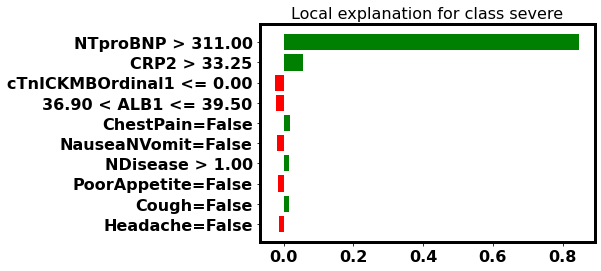
\includegraphics[width=\textwidth]{figures/chapter_interp/lime_dt_2.png}
    \caption{Decision Tree}
    \label{fig:lime_dt_2}
\end{subfigure}
\hfill
\begin{subfigure}[b]{\textwidth}
    \centering
    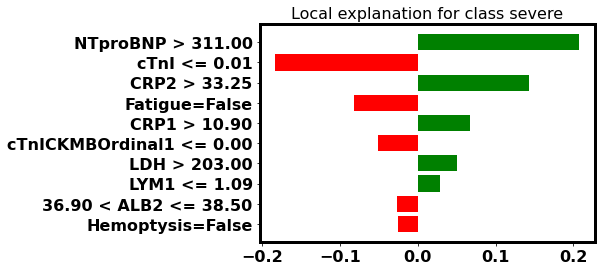
\includegraphics[width=\textwidth]{figures/chapter_interp/lime_rf_2.png}
    \caption{Random Forests}
    \label{fig:lime_rf_2}
\end{subfigure}
\end{figure}
\vfill

\clearpage

\null
\vfill

\begin{figure}[H] \ContinuedFloat
\begin{subfigure}[b]{\textwidth}
    \centering
    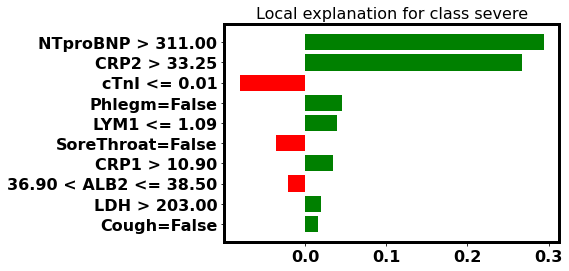
\includegraphics[width=\textwidth]{figures/chapter_interp/lime_xgbc_2.png}
    \caption{Gradient Boosted Trees}
    \label{fig:lime_xgb_2}
\end{subfigure}
\begin{subfigure}[b]{\textwidth}
    \centering
    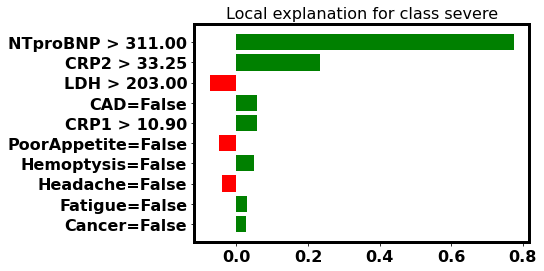
\includegraphics[width=\textwidth]{figures/chapter_interp/lime_nn_2.png}
    \caption{Neural Networks}
    \label{fig:lime_nn_2}
\end{subfigure}
\caption{LIME Explanation (\textbf{False-Positive Patient No.2}): Features in green have a positive contribution to the prediction (increasing the probability of turning severe), and features in red have a negative effect on the prediction (decreasing the probability of turning severe)}
\label{fig:lime_2}
\end{figure}

\vfill

\clearpage

\begin{sidewaysfigure}
\centering
\begin{subfigure}[b]{1.0\textheight}
    \centering
    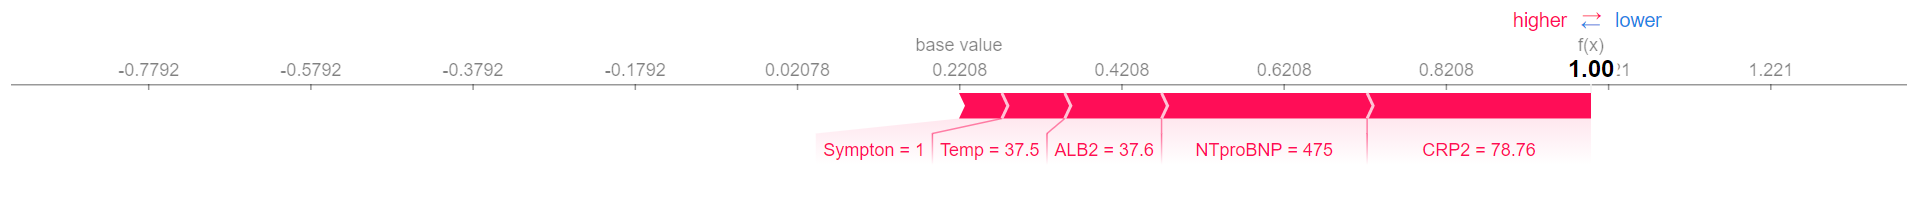
\includegraphics[width=\textheight]{figures/chapter_interp/shap_dt_2.png}
    \caption{Decision Tree}
    \label{fig:shap_dt_2}
\end{subfigure}
\hfill
\begin{subfigure}[b]{1.0\textheight}
    \centering
    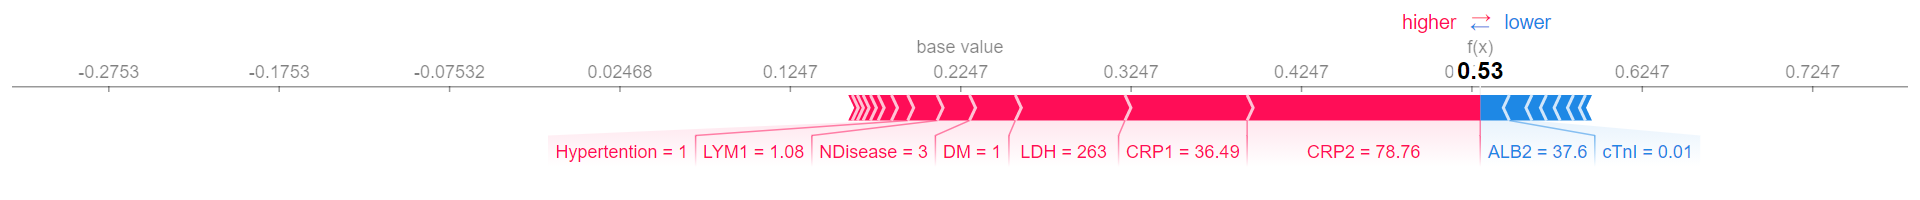
\includegraphics[width=\textheight]{figures/chapter_interp/shap_rf_2.png}
    \caption{Random Forests}
    \label{fig:shap_rf_2}
\end{subfigure}
\hfill
\begin{subfigure}[b]{1.0\textheight}
    \centering
    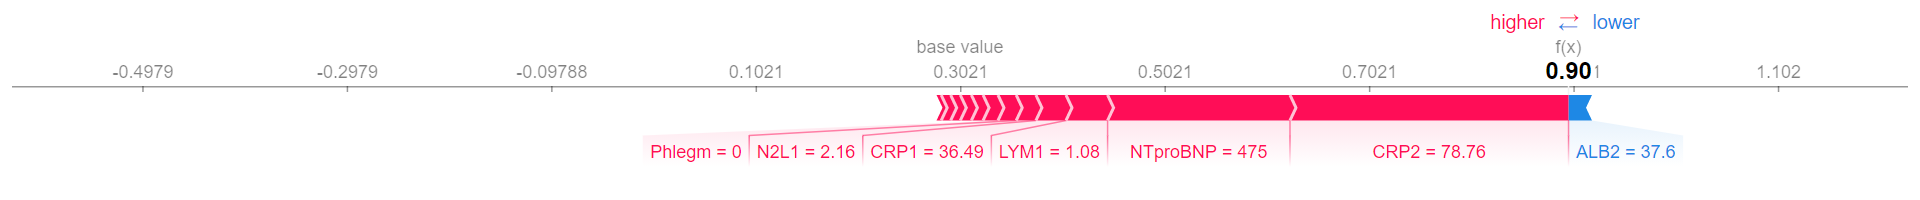
\includegraphics[width=\textheight]{figures/chapter_interp/shap_xgbc_2.png}
    \caption{Gradient Boosted Trees}
    \label{fig:shap_xgbc_2}
\end{subfigure}
\hfill
\begin{subfigure}[b]{1.0\textheight}
    \centering
    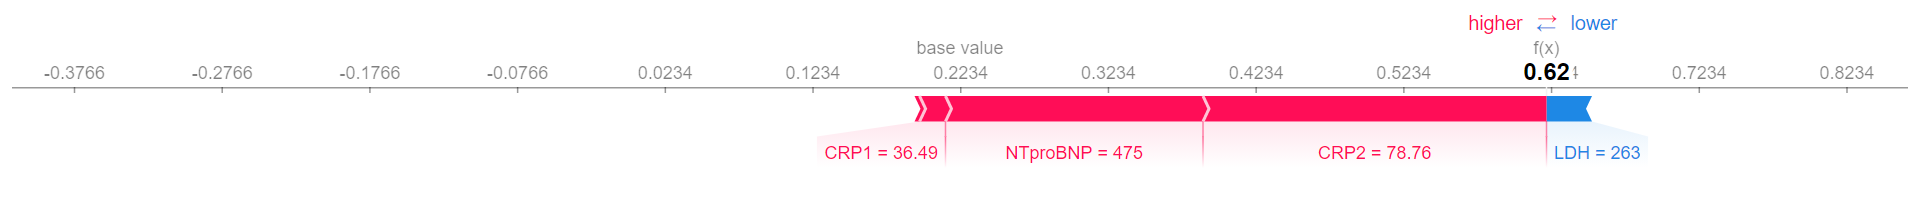
\includegraphics[width=\textheight]{figures/chapter_interp/shap_nn_2.png}
    \caption{Neural Networks}
    \label{fig:shap_nn_2}
\end{subfigure}
\hfill
\caption{SHAP Explanation (\textbf{False-Positive Patient No.2}): Features pushing the prediction to be higher (severe) are shown in red,  and those pushing the prediction to be lower (normal) are in blue.}
\label{fig:shap_2}
\end{sidewaysfigure}

\clearpage
\subsection{Evaluating Interpretation}

Though we do find some indicative symptoms of COVID-19 through model interpretation, they are confirmed credible because these interpretations are corroborated by medical research. If we use the interpretation to understand a new virus at the early stage of an outbreak, there will be less evidence to support our interpretation. Thus we use Monoitinicity and Faithfulness to evaluate different interpretations using IBM AIX 360 toolbox \citep{aix360-sept-2019}. The decision tree only provides a binary prediction (0 or 1) rather than a probability between 0 and 1, so it cannot be evaluated using Monotonicity and Faithfulness.

\begin{table}[H]
\centering
\begin{tabular}{@{}ccc@{}}
\toprule
Models   & LIME & SHAP \\ \midrule
Random Forests & 0.37  & 0.59      \\
Gradient Boosted Trees & 0.46 & 0.49 \\
Neural Networks & 0.45 & 0.33 \\ \bottomrule
\end{tabular}
\caption{Failthfulness Evaluation}
\end{table}

Faithfulness (ranging from -1 to 1) reveals the correlation between the importance assigned by the interpretability algorithm and the effect of each attribute on the performance of the model. All of our interpretations receive good faithfulness scores, and SHAP receives a higher faithfulness score than LIME on average. The interpretation by SHAP receives better results because the Shapley value is calculated by removing the effect of specific features which is similar to how faithfulness is computed, so SHAP is more akin to faithfulness.

\begin{table}[H]
\centering
\begin{tabular}{@{}ccc@{}}
\toprule
Models   & LIME & SHAP \\ \midrule
Random Forests & False  & False      \\
Gradient Boosted Trees & 22\% True & 22\% True \\
Neural Networks & False & False \\ \bottomrule
\end{tabular}
\caption{Monotonicity Evaluation}
\end{table}

% \color{blue}
As for monotonicity, most interpretation methods receive a False though we do find valuable conclusions from interpretations. The difference between faithfulness and monotonicity is that faithfulness incrementally removes each of the attributes, while monotonicity incrementally adds each of the attributes. By incrementally adding each attribute, initially, the model may not be able to make correct predictions with only one or two features, but this does not mean these features are not important. Evaluation metrics for different interpretation methods is still an active research direction, and our results may hopefully stimulate further research on the development of better evaluation metrics for interpreters.

% \par
% From these results, we can see that the scores of different metrics are heavily dependent on how similarly they are calculated using an interpretation method, which suggests that these metrics can be biased. As a result, it may be more reliable to manually check the fidelity of different interpretations in comparison with prior medical knowledge.

% The evaluation metrics for different interpretation methods is still an active research direction, thus it's an open question what is the best way to measure interpretations. 
\color{black}

\subsection{Summary}

In this section, the interpretation of four different machine learning models reveals that N-Terminal pro-Brain Natriuretic Peptide (NTproBNP), C-Reaction Protein (CRP), and lactic dehydrogenase (LDH), lymphocyte (LYM) are the four most important biomarkers that indicate the severity level of COVID-19 patients. In the next section, we further validate our methods on two datasets to corroborate our proposal.

% \clearpage

\section{Validation on other datasets}

At the initial outbreak of the pandemic, our research leverages a database consisting of patients with confirmed SARS-CoV-2 laboratory tests between 18th January 2020, and 5th March 2020, in Zhuhai, China, and reveals that an increase in NTproBNP, CRP, and LDH, and a decrease in lymphocyte count indicates a higher risk of death. However, the dataset has a limited record of 92 patients which may not be enough to support our proposal. Luckily, and thanks to global cooperation, we do have access to larger datasets. In this section, we further validate our methods on two datasets, one with 485 infected patients in Wuhan, China\citep{Yan2020}, and the other with 5644 confirmed cases from the Hospital Israelita Albert Einstein, at São Paulo, Brazil from Kaggle.

\subsection{Validation on 485 infected patients in China}

The medical record of all patients in this dataset was collected between 10th January and 18th February 2020, within a similar date range as our dataset. Yan et al. construct a dedicated simplified and clinically operable decision model to rank 75 features in this dataset, and the model demonstrates that three key features, lactic dehydrogenase (LDH), lymphocyte (LYM), and high-sensitivity C-reactive protein (hs-CRP) can help to quickly prioritize patients during the pandemic, which is consistent with our interpretation in Table \ref{tab:important_feature}.

Findings from the dedicated model are consistent with current medical knowledge. The increase of hs-CRP reflects a persistent state of inflammation \citep{pmid19411291}. The increase of LDH reflects tissue/cell destruction and is regarded as a common sign of tissue/cell damage, and the decrease of lymphocyte is supported by the results of clinical studies \citep{chen2020epidemiological}.

\begin{figure}[H]
% \setcounter{figure}{3}
\centering
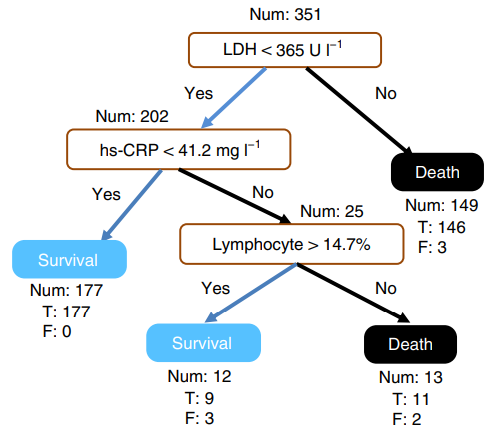
\includegraphics[width=0.6\textwidth]{figures/chapter_interp/nature_dt.png}
\caption{A decision rule using three key features and their thresholds in
absolute value. Num, the number of patients in a class; T, the number of
correctly classified; F, the number of misclassified patients. \citep{Yan2020}}
\end{figure}

Our methods reveal the same results without taking efforts to design a dedicated interpretable model but can be more prompt to react to the pandemic. During pandemic outbreak, a prompt reaction that provides insights on the new virus could save lives and time. 

\subsection{Validation on 5644 infected patients in Brazil}

Our approach obtains the same result on the dataset with 92 patients from Zhuhai, China, and a medium-size dataset with 485 patients from Wuhan, China. Besides, we further validate our approach on a larger dataset with 5644 patients in Brazil, from Kaggle.

This dataset consists of 111 features including anonymized personal information, laboratory virus tests, urine tests, venous blood gas analysis, arterial blood gases, blood routine test, among other features. All data were anonymized following the best international practices and recommendations. The difference between this dataset and ours is that all data are standardized to have a mean of zero and a unit standard deviation, thus the original data range that contains clinical meaning is lost. Still, the most important medical indicators can be extracted using interpretation methods.

\begin{table}[H]
\centering
\begin{tabular}{@{}ll@{}}
\toprule
Feature & Value\\ 
\midrule
SARS-Cov-2 test result & 1 \\
Patient Age Quantile & 14.00\\
Hematocrit  & 0.92\\
% Hemoglobin & 0.48\\
Platelets  & -1.26\\ 
Mean platelet volume  & 0.79\\ 
% Red blood Cells & 1.32\\
% Lymphocytes  & 0.57\\
Mean corpuscular hemoglobin concentration (MCHC)  & -0.65\\
Leukocytes & -1.47\\
Basophils  & -1.14\\
% Mean corpuscular hemoglobin (MCH) & -1.44\\
Eosinophils & -0.83\\
% Mean corpuscular volume (MCV) & -1.19\\
Monocytes & 0.96\\  
% Red blood cell distribution width (RDW)  & 0.97\\ 
% Neutrophils & -0.44\\ 
Proteina C reativa mg/dL & 0.236\\ 
\bottomrule
\label{tab:kaggle}
\end{tabular}
\caption{Patient No.0 in the Kaggle Dataset}
\end{table}

% \color{blue}
Following the same approach, a preprocessing is applied on the dataset that removes irrelevant features such as patients' intention to the ward level, and features that have less than 100 patient's record, for instance, urine tests and aerial blood gas tests. On the other hand, patients that have less than 10 records are dropped, because these records do not provide enough information. After preprocessing, we have a full record of 420 patients with 10 features.
\color{black}

\begin{table}[H]
\centering
\begin{tabular}{cccccc}
\toprule
Classifier    & CV & \multicolumn{3}{c}{Test Set} & 95\% CI \\ \midrule
              & F1               & Precision  & Recall  & F1    &\\
Decision Tree & 0.37             & 0.88       & 0.75    & 0.71  & 0.098\\
Random Forests & 0.37             & 0.90       & 0.50    & 0.67  & 0.089\\
Gradient Boosted Trees  & 0.56    & 0.90       & 0.75    & 0.59 & 0.089\\
Neural Networks       & 0.38             & 0.90       & 0.50    & 0.67 & 0.089\\ \bottomrule
\label{tab:kaggle_models}
\end{tabular}
\caption{Classification Results (Kaggle)}
\end{table}

After training and interpreting four different models, decision tree, random forests, gradient boosted trees, and neural networks, the most important features are identified and listed in table \ref{tab:important_feature_kaggle}. The three most common indicative features are leukocytes, eosinophils, and platelets.

According to medical research, patients with increased leukocyte count are more likely to develop critically illness, more likely to admit to an ICU, and have a higher rate of death \citep{zhao2020clinical}. Du et al. noted that at the time of admission, 81\% of the patients had absolute eosinophil counts below the normal range in the medical records of 85 fatal cases of COVID-19\citep{du2020clinical}. Wool G.D. and Miller J.L. discovered that COVID-19 is associated with increased numbers of immature platelets which could be another mechanism for increased clotting events in COVID-19\citep{wool2021impact}.

\begin{table}[H]
\centering
\begin{tabular}{@{}ccc@{}}
\toprule
Model                   & Most Important Features \\ \midrule
Decision Tree           & Leukocytes, Eosinophils, Patient age quantile      \\
Random Forest           & Leukocytes, Eosinophils, Platelets        \\
Gradient Boosted Trees  & Patient age quantile, Hematocrit, Platelets  \\
Neural Networks         & Leukocytes, Platelets, Monocytes          \\  \bottomrule
\end{tabular}
\caption{Five most important features (Kaggle)}
\label{tab:important_feature_kaggle}
\end{table}

% \color{blue}
In addition, the two datasets collectively reveal that elderly people are more susceptible to the virus. The significant feature NTproBNP in the Chinese dataset is often used to diagnose or rule out heart failure which is more likely to occur in elderly people. And patients that have abnormally low levels of platelets are more likely to be older, male as well \citep{wool2021impact}.
\color{black}

To further validate our interpretation, faithfulness and monotonicity are calculated and listed in tables \ref{kaggle_faith} and \ref{kaggle_mono}. Similarly, our interpretations are consistent with medical knowledge and receive a good faithfulness score, but receive a worse score on monotonicity because the calculation procedure of monotonicity is contrary to faithfulness.

\begin{table}[H]
\centering
\begin{tabular}{@{}ccc@{}}
\toprule
Models   & LIME & SHAP \\ \midrule
Random Forests & 0.71  & 0.82      \\
Gradient Boosted Trees & 0.61 & 0.72 \\
Neural Networks & 0.25 & 0.42 \\ \bottomrule
\end{tabular}
\caption{Failthfulness Evaluation (Kaggle)}
\label{kaggle_faith}
\end{table}

\begin{table}[H]
\centering
\begin{tabular}{@{}ccc@{}}
\toprule
Models   & LIME & SHAP \\ \midrule
Random Forests & False  & False      \\
Gradient Boosted Trees & True & False \\
Neural Networks & False & False \\ \bottomrule
\end{tabular}
\caption{Monotonicity Evaluation (Kaggle)}
\label{kaggle_mono}
\end{table}

\clearpage

\null
\vfill

\begin{figure}[H]
% \setcounter{figure}{4}
\centering
\begin{subfigure}[b]{\textwidth}
    \centering
    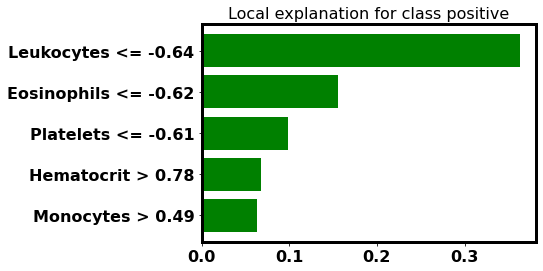
\includegraphics[width=\textwidth]{figures/chapter_interp/lime_kaggle_dt.png}
    \caption{Decision Tree}
    \label{fig:lime_kaggle_dt}
\end{subfigure}
\hfill
\begin{subfigure}[b]{\textwidth}
    \centering
    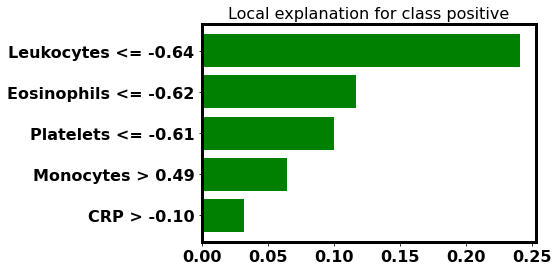
\includegraphics[width=\textwidth]{figures/chapter_interp/lime_kaggle_rf.png}
    \caption{Random Forests}
    \label{fig:lime_kaggle_rf}
\end{subfigure}
\end{figure}
\vfill

\clearpage

\null
\vfill

\begin{figure}[H] \ContinuedFloat
\begin{subfigure}[b]{\textwidth}
    \centering
    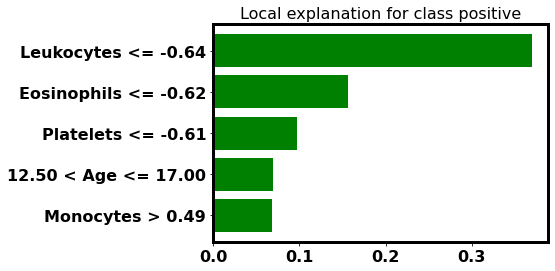
\includegraphics[width=\textwidth]{figures/chapter_interp/lime_kaggle_xgbc.png}
    \caption{Gradient Boosted Trees}
    \label{fig:lime_kaggle_xgbc}
\end{subfigure}
\hfill
\begin{subfigure}[b]{\textwidth}
    \centering
    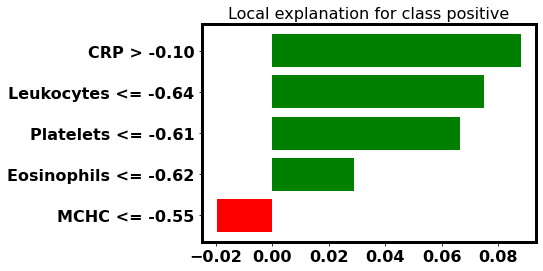
\includegraphics[width=\textwidth]{figures/chapter_interp/lime_kaggle_nn.png}
    \caption{Neural Networks}
    \label{fig:lime_kaggle_nn}
\end{subfigure}
\hfill
\label{fig:kaggle_lime}
\caption{LIME Explanation (\textbf{Kaggle Patient 0}): Features in green have a positive contribution to the prediction (increasing the probability of turning severe), and features in red have a negative effect on the prediction (decreasing the probability of turning severe)}
\end{figure}
\vfill

\clearpage

\section{Conclusion}

In this research, through the interpretation of four different machine learning models, we reveal that N-Terminal pro-Brain Natriuretic Peptide (NTproBNP), C-Reaction Protein (CRP), and lactic dehydrogenase (LDH), lymphocyte (LYM) are the four most important biomarkers that indicate the severity level of COVID-19 patients. Our findings are consistent with medical knowledge and recent research that exploits dedicated models. We further validate our methods on a large open dataset from Kaggle and unveil leukocytes, eosinophils, and platelets as three indicative biomarkers for COVID-19.

The pandemic is a race against time. Using interpretable machine learning, medical practitioners can incorporate insights from models with their prior medical knowledge to promptly reveal the most significant indicators in early diagnosis and hopefully win the race in the fight against the pandemic.

% \clearpage

% \printbibliography[
%   keyword={chapter_defence}, heading=subbibintoc, resetnumbers=true
% ]
